\chapter{Trabalhos Analisados}
\label{cap:trabalhos-analisados}

Esse capítulo tem como objetivo destacar as principais pesquisas realizadas com
o objetivo de expandir as abstrações de processos. Para a seleção dos trabalhos
aqui apresentados, o autor levou em consideração os seguintes aspectos:
quantidade de citações dos trabalhos, implementação da proposta em um SO e
pesquisas que tenham a abstração de processos como objeto de estudo. Por uma
questão organização, esse trabalho subdivide as pesquisas usando o critério da
implementação. Sem entrar em detalhes, as três categorias são:
\textit{Implementação Estrutural Leve, Implementação Estrutural Pesada e
Implementação Independente}. Por fim, essa seção visa fornecer as bases para a
discussão apresentada no Capitulo
\ref{cap:analise-sobre-abstracoes-de-processos}, tema central desse trabalho.

\section{Implementação Estrutural Leve}

Chamamos de \textit{Implementação estrutural leve} toda proposta que não altera
diretamente o núcleo do SO, isso faz com que a proposta tenha uma grande chance
de ser incorporada em um contexto de um SO de produção e ao mesmo tempo geram
pouco impacto geral no SO. Normalmente, implementações leves utilizam
artifícios de \emph{device drivers} (Veja \ref{sec:dd}), o que torna simples de
desenvolver e testar novas propostas.

\subsection{Dune}

Como mostrado na Seção \ref{sec:virtualizacao}, o conceito de virtualização já
é amplamente conhecido e adotado pela indústria; dentre os recentes avanços
destacam-se a virtualização via hardware proporcionada pelos processadores
modernos. O mecanismo de virtualização é utilizada com o objetivo de fornecer
abstrações para a criação de máquinas virtuais. Com esse conceito em mente,
\cite{belay} decidiram dar outra utilidade para esses recursos de hardware:
fornecer processos ao invés de máquinas virtuais.

Os autores defendem que uma ampla variedade de aplicações podem tirar proveito
do acesso a certos recursos que são apenas disponíveis ao kernel. Dentre as
aplicações que podem comprovadamente ganhar algum desempenho ao obter acesso
direto ao hardware, destacam-se:

\begin{itemize}
  \item \textbf{Garbage Collection (GC)}: O GC pode ganhar desempenho caso
        tenha como controlar diretamente o hardware de paginação, como
        \cite{pauseless} demostraram em seu trabalho;
  \item \textbf{Process Migration}: Programas no espaço de usuário podem tirar
        proveito do acesso direto as faltas de páginas e chamadas de sistema.
\end{itemize}

Não obstante, fornecer o acesso direto aos recursos de hardware de forma segura
e gerenciável não é uma tarefa trivial uma vez que requer mudanças na forma
como o espaço de usuário e o espaço do Kernel interagem. Além disso, alterações
no Kernel são consideradas invasivas e perigosas uma vez que uma modificação
feita de forma errada pode comprometer toda a estabilidade do sistema. Outra
alternativa para dar acesso de hardware para aplicações é por meio de imagens
de máquina virtual, assim uma aplicação consegue acesso seguro aos recursos de
hardware através da interface de virtualização. Uma desvantagem desta abordagem
é que ela tem pouca integração com o SO da máquina \emph{host} o que impede um
processo de obter ganhos de desempenho.

\cite{belay} oferecem uma alternativa que consiste em utilizar a abstração de
virtualização disponível nos processadores modernos de forma a fornecer um novo
tipo de processo que executa no chamado \emph{Dune Mode} (modo Dune). Tal modo
é um estado irreversível no qual o processo indica explicitamente que quer
entrar; nesse modo o processo passa a ter acesso direto, por meio dos recursos
de virtualização, a modos de operação com maior privilégio, registradores de
memória virtual, tabelas de páginas, interrupções, exceções e vetores de
chamada de sistema. Para auxiliar a aplicação no espaço de usuário a interagir
com tais recursos, os autores criaram uma biblioteca chamada \emph{libDune} que
na utilização das novas funcionalidades.

Dentre as vantagens que o Dune promete, destacam-se o fato de que no modo Dune
o processo comporta-se como um processo normal com a diferença de que este
utiliza a instrução VMCALL para fazer chamadas de sistema. Além disto, devido
ao fato de que o Dune não tem por objetivo fornecer máquinas virtuais este
consequentemente consegue ser mais simples e rápido. As aplicações que se
adequam ao uso desse modelo podem obter melhorias de desempenho e isolamento.

Para implementar o Dune, os pesquisadores utilizaram os processadores Intel com
suporte para a tecnologia VT-x (Veja \ref{sec:vtx}) e parte do código do KVM já
disponível no Kernel Linux. O Dune apresenta três tipos de instruções
privilégiadas para os processos:

\begin{itemize}
  \item \textbf{Exceções}:  As instruções LIDT, LTR, IRET, STI e CLI são
        expostas diretamente para os processos. Note que emulações, depuração e
        rastreamento de desempenho são aplicações que podem tirar proveito
        desta característica uma vez que o Dune pode reduzir consideravelmente
        a sobrecarga em entregar exceções. Isso se deve ao fato que o Dune
        consegue entregar exceções diretamente para o hardware de forma segura
        (encapsulado pelo hardware de virtualização);
  \item \textbf{Memória Virtual}: As instruções \texttt{MOV CRn, INVLPG} e
        \texttt{INVPCID} são apresentadas para o processo Dune. O acesso
        flexível a memória virtual pode ser benéfico para aplicações que fazem
        \emph{checkpointing}, GC, compressão de dados nas páginas e memória
        compartilhada distribuída. O Dune traz melhorias para o acesso a
        memória virtual expondo as entradas da tabela de páginas para as
        aplicações, isso permite que elas controlem a tradução de endereços,
        permissão de acesso, bits globais e modifiquem/acessem as páginas com
        simples referências. Por fim, o Dune também da a habilidade para
        controlar as invalidações da TLB manualmente o que pode ser vantajoso
        para alguns tipos de aplicações;
  \item \textbf{Modos privilégiados}: As instruções \texttt{LGDT} e
        \texttt{LLDT} permitem que o Dune exponha os modos privilégiados de
        forma segura. O Dune expõe esse modos de forma eficiente e segura por
        que o VMX non-root mantém o seu próprio conjunto de anéis privilégiados
        (Veja \ref{sec:vtx}).
\end{itemize}

A Figura \ref{fig:dune_architecture} ilustra a arquitetura do Dune. O Dune
estende o Kernel como um modulo que habilita o VT-x, colocando o mesmo em um
modo VMX root. Assim processos usando Dune tem acesso seguro e garantido para
hardware privilégiado utilizando o VMX non-root mode. O módule Dune intercepta
os VM exits, o único motivo para o processo acessar o kernel e realizar
qualquer ação. Repare que o Dune é aplicado de forma seletiva aos processos que
de fato precisam deles, isto significa que um processo que não usa o Dune não é
afetado. A transição de um processo normal para o modo Dune ocorre por meio de
uma chamada de \texttt{ioctl} no dispositivo \texttt{/dev/dune}, repare que ao
entrar em tal modo o processo não pode retornar ao modo anterior. Sempre que um
processo Dune faz um \texttt{fork()}, o processo filho não incia em modo Dune,
contudo pode reentrar caso queira.

\begin{figure}[!h]
  \centering
  \includegraphics[width=0.6\textwidth]{dune_architecture} 
  \caption{A arquitetura do Dune, imagem baseada em \citep{belay}}
  \label{fig:dune_architecture}
\end{figure}

Seção \ref{sec:virtualizacao} apresentamos as principais propriedades dos VMMs,
com o objetivo de deixar claro as diferenças entre o VMMs e as características
de hardware expostas pelo Dune, destacamos as principais diferenças:

\begin{itemize}
  \item No Dune, o mecanismo de \textit{hypercall} invocam
        \textit{system calls} comuns do Linux;
  \item Apenas características de hardware que podem ser acessadas diretamente
        sem a intervenção do VMM são disponíveis para a aplicação, nos casos em
        que não é possível executar dada operação, o Dune retorna o controle
        para o SO;
  \item Podemos limitar as diferenças entre \textit{guest} e \textit{host} uma
        vez que processos usando Dune tem uma interface próxima da de hardware;
  \item No Dune é preciso configurar o EPT para refletir o endereço do espaço
        de usuário.
\end{itemize}

\subsection{Shreds}

Existe uma categoria de ataques chamadas de "abusos intra-processos de conteúdo
de memória", na qual o invasor busca acessar determinado tipo de conteúdo
sensível na memória (e.g., dados secretos) ou uma região de código crítica
(e.g., funções privilégiadas) \citep{shreds}. O roubo deste tipo de dados
acontece por meio da introdução de algum código injetado ou por meio de alguma
biblioteca maliciosa que permite acessar alguma região da memória não protegida
da vítima. Note que bibliotecas maliciosas são especialmente perigosas uma vez
que estas podem executar funções privilegiadas que são de fato parte do
processo, por exemplo, a função \texttt{dlopen}. Por fim, se o atacante
conseguir o acesso a memória, este pode ler todos os dados buscando por outras
informações.

\cite{shreds} defendem que o problema de segurança referente aos ataques
intra-processos decorrem da falta de controle-fino e eficiente do conteúdo de
sensível da memória; além disto, eles argumentam que séria benéfico se tais
funcionalidades fossem disponibilizadas para os programados.  Para resolver tal
problema os autores apresentam uma nova abstração de processos que cria uma
nova unidade de execução chamada de \emph{shreds}, esta tem associado a si um
fragmento de memória protegida denominada de \emph{shred-private pool
(s-pool)}. O tamanho do segmento de memória criado tem o seu tamanho variável
dependendo da necessidade da aplicação, além disso este comporta-se de forma a
existir apenas durante o momento em que é necessário para um pedaço da
aplicação. A implementação do \emph{shreds} é baseado em três pilares: uma API
para o usuário conseguir utilizar facilmente as funcionalidade oferecidas, um
\emph{toolchain} de compilação que verifica a correta utilização dos
\emph{shreds} (\emph{S-compiler}) e um módulo Linux que faz o gerenciamento da
memória (\emph{S-driver}).

O \emph{shreds} foi projetado buscando três propriedades que visam garantir
segurança, são elas:

\begin{itemize}
  \item \textbf{Acesso exclusivo para s-pool:} Um \emph{s-pool} só é acessível
        para o \emph{shreds} associado a si;
  \item \textbf{Evitar vazamentos na entrada e saída:} Dados carregados em um
        \emph{s-pool} não podem ser copiados ou exportado sem ter uma operação
        de limpeza antes;
  \item \textbf{Execuções não desviáveis:} O fluxo de execução não pode ser
        alterado para fora do \emph{shreds}.
\end{itemize}

Para melhor entender como o \emph{shreds} se comporta, veja a Figura
\ref{fig:shreds} ilustrando uma aplicação que lida com uma senha (dado
sensível) e o código que manipula tal dado. A aplicação possui uma thread que
comporta-se da forma padrão, contudo, ao ter que lidar com um dado sensível ela
faz uma chamada para uma função da API fornecida pelo \emph{shreds},
\texttt{shred\_enter()}. Ao realizar a chamada para a função o fluxo de
execução entra em um modo seguro no qual o \emph{shreds} gerência o acesso a
memória e garante que os dados são isolados no sistema. Por fim, após realizar
a operação na região protegida a aplicação do usuário chama
\texttt{shred\_exit()}. Para utilizar a proposta dos autores, é preciso alterar
as aplicações alvo.

\begin{figure}[!h]
  \centering
  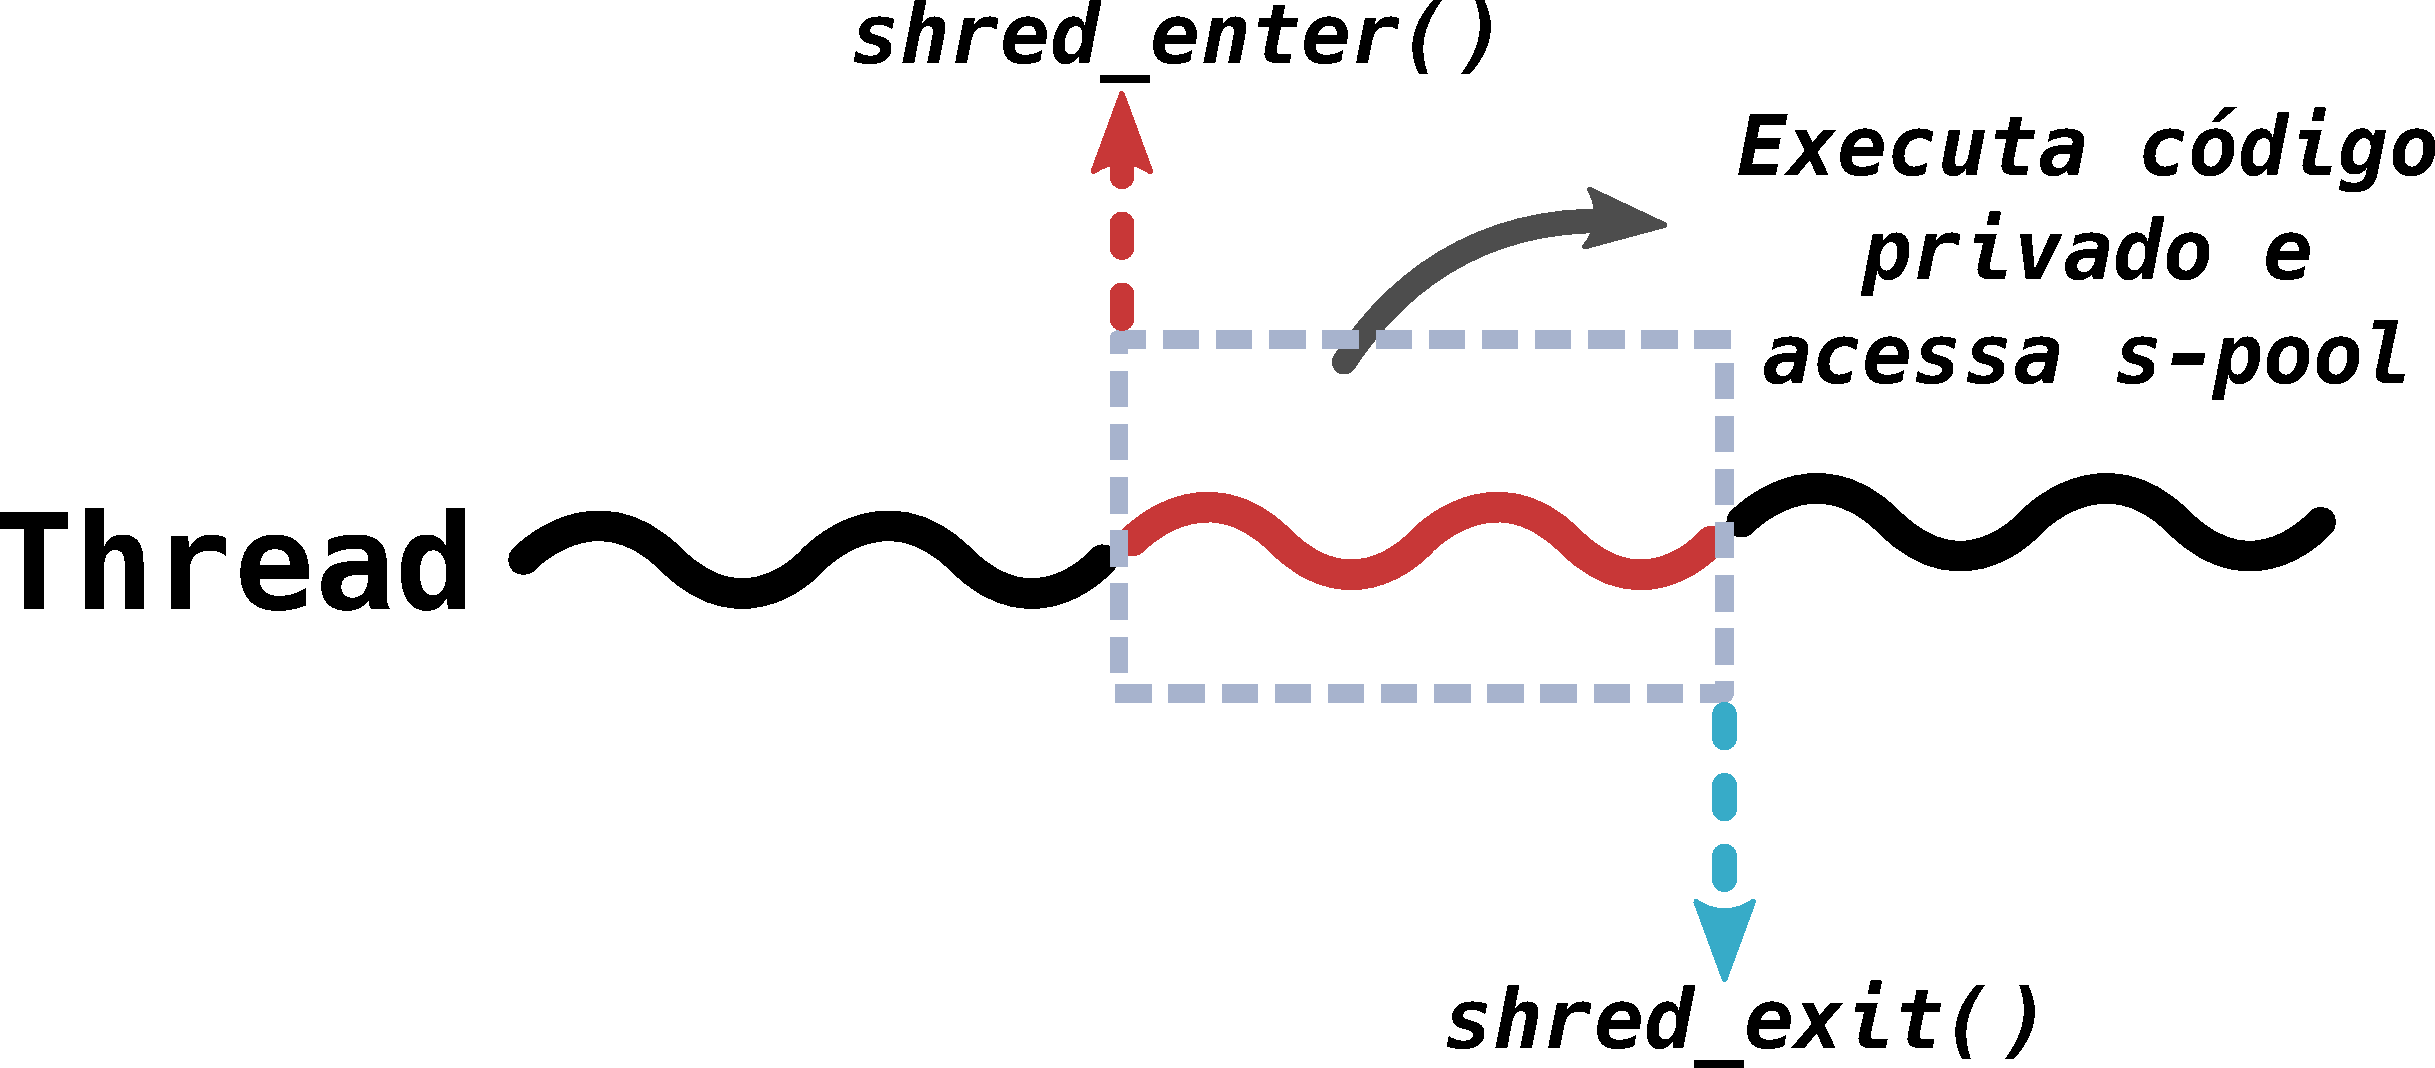
\includegraphics[width=0.6\textwidth]{shreds} 
  \caption{Funcionamento geral do shreds}
  \label{fig:shreds}
\end{figure}

A API fornecida pelo \emph{shred} consiste de apenas quatro funções:

\begin{itemize}
  \item \texttt{shred\_enter()}: Inicia a execução na thread atual, faz uma
        troca para execução em uma stack alocada para um \textit{s-pool} e
        espera um descritor para um pool;
  \item \texttt{shred\_exit()}: Suspende o shred chamado, revoga as permissões
        de acesso da thread atual sobre o s-pool e recupera a stack de execução
        original;
  \item \texttt{spool\_alloc()}: Alocar memória para o s-pool associado com a
        thread;
  \item \texttt{spool\_free()}: Apaga a memória alocada.
\end{itemize}

Para garantir que as regras de utilização da API sejam seguidas o
\emph{S-compiler} realiza verificações e instrumentações para evitar falhas que
abram brechas de segurança.

Para este trabalho, a parte mais importante do \emph{shred} é o \emph{S-driver}
que consiste em um módulo do Linux responsável por gerir as \emph{shreds} e
\emph{s-pools}. A implementação dessa técnica é baseada em domínios de memória
do ARM (Seção \ref{sec:outros_mecanismos_memoria}), contudo, dado que está
tecnologia não foi projeta para os propósitos sugeridos pelo \emph{shreds} a
mesma apresenta duas limitações:

\begin{itemize}
  \item O ARM fornece apenas 16 domínios, isso impede que se crie um domínio
        para cada \emph{s-pool} uma vez que este pode crescer de forma
        indeterminada;
  \item O controle de acesso a memória é extremamente limitado.
\end{itemize}

A solução adotada pelos autores foi implementar um mecanismo que multiplexa os
domínios e introduz identidades dentro da lógica de acesso. Para permitir que
uma aplicação tenha várias \emph{shreds} o \emph{S-driver} utiliza os domínios
de forma temporária e rotacionando as identidades de segurança para o
\emph{s-pool}. Toda vez que uma \emph{shreds} inicia ou retoma a sua execução
em uma $CPU_i$ o \emph{S-driver} atribui um \emph{s-pool} associado a um
domínio $Dom_i$, isto faz com que uma \emph{shred} consiga acessar o seu
\emph{s-pool} enquanto outra threads concorrente não consegue acessar. Quando o
\emph{shred} finaliza ou tem a sua execução parada em detrimento de outro
processo, o \emph{S-driver} muda o domínio prevenindo que outro processo
consiga acessar a região de memória. Note que o driver permite ou rejeita o
acesso a um \emph{s-pool} baseado na CPU, isso faz com que mesmo que um código
malicioso consiga executar em paralelo com o \emph{shred} ele não consiga ter
acesso ao \emph{s-pool} sem que seja disparada uma falha de domínio.

Uma das funcionalidades fornecidas pelo \emph{shread} é a habilidade de
permitir fazer cópias para regiões de memória não protegidas de forma segura
(e.g., atribuir dados de um \emph{s-pool} para uma variável local). Note que
para realizar tal procedimento é preciso acessar uma stack regular que pode ter
sido atacada e conter um código mal-intencionado, o que violaria toda proteção
fornecida pelo \emph{s-compiler} e \emph{S-driver}. Para prevenir que dados
sejam vazados via stack, o \emph{S-driver} cria uma stack segura para cada
\emph{shred} alocada partindo do \emph{s-pool} associado a si.

\section{Implementação Estrutural Pesada}

As \textit{Implementações Estruturais Pesadas} são aquelas que alteram
diretamente o núcleo do SO, essa abordagem traz vantagens e desvantagens que
devem ser consideradas antes de serem adotadas. Por um lado, alterações diretas
no núcleo são mais flexíveis em termos de possibilidade de acesso aos recursos
disponíveis do SO. Por outro lado, alterações no núcleo são complicadas uma vez
que podem afetar toda a estabilidade do sistema e são extremamente complexas de
serem feitas uma vez que demandam profundo conhecimento do SO em questão.

\subsection{Wedge}

Existe um princípio chamado de \emph{"Princípio do Menor Privilégio"} que diz:

\begin{quote}
Divida o código em compartimentos na qual cada um vai executar com o menor
privilégio para completar a sua tarefa. Essa abordagem previne contra ataques
e também previne bugs que levam ao vazamento de dados.
\citep{protectionprinciple}
\end{quote}

Apesar deste princípio ter sido apresentado em 1975 e ser amplamente aceito,
nota-se que várias aplicações que tem acesso a Internet (um ponto de acesso
para o mundo) não buscam atender a este fundamento e acabam abrindo
potencias pontes de vazamento de dados ou falhas de segurança. Alguns
pesquisadores defendem que esse problema surge do fado de que os SO atuais
garantem privilégios por padrão. Isto significa que impor limites requer mais
esforço por parte do programador e também é propenso a erros.

A chamada de sistema \texttt{fork} ilustra a característica de garantir
privilégios por padrão. Quando o processo pai cria um filho, este recebe uma
cópia praticamente exata do pai. Se o programador desejar restringir o nível de
acesso do processo filho é preciso realizar uma série de operações manuais que
não garantem que nenhum aspecto tenha sido ignorado.

\cite{wedge} buscaram resolver tal problema mudando o princípio atual de
garantir privilégio por padrão, para negar privilégios por padrão. Nessa
abordagem o programador deve indicar explicitamente que deseja garantir
permissões adicionais. Os autores alteraram o GNU/Linux para que este
suportasse a remoção de permissões por patrão e chamaram o modelo proposto por
eles de \emph{Wedge}. O \emph{Wedge} fornece um conjunto de primitivas de
programação para permitir criar componentes com semântica de negar permissão
por padrão tornando o acesso mais restrito. Para isto, o \emph{Wedge} oferece
um esquema simples e flexível de marcação (\emph{tagging}) da memória o que
permite ao programador alocar objetos de memória distintas com a mesma
marcação.

O \emph{Wedge} permite que o programador crie um número arbitrário de
componentes, cada um sem privilégios por padrão, mas existem mecanismos que
permitem o controle fino. Neste sentido o \emph{Wedge} busca se assemelhar as
primitivas atuais para facilitar a sua adoção e para que seja simples a
introdução delas em aplicações legadas. A proposta é constituída de três
primitivas: \emph{Sthread}, \emph{Tagged Memory}, and \emph{callgates}. O
acesso a todas essas primitivas é feito via chamada de sistemas.

Uma \emph{Sthread} define um compartimento dentro de uma aplicação, o
programador pode atribuir permissão de acesso para a memória e outros recursos
por meio das \emph{sthreads}. Estas consistem de uma thread de controle e
políticas de segurança associado a si, que especificam:

\begin{itemize}
	\item As marcações de memória que o \emph{sthread} pode acessar e a permissão
				para cada um (leitura, leitura-escrita e \textit{copy-on-write});
	\item Os descritores de arquivo que a \emph{sthread} pode acessar e as
				permissões de cada (leitura, escrita, leitura-escrita);
	\item Os \emph{callgates} que a \emph{sthread} pode chamar;
	\item O \emph{Unix user id}, o \emph{root directory} e o \emph{SELinux}.
\end{itemize}

Uma nova \emph{sthread} não mantém as permissões de acesso por padrão, a não
ser pelo \emph{snapshot} intocado do \emph{copy-on-write} acessado. Note que o
novo componente não tem permissão para acessar qualquer outra memória ou mesmo
descritor de arquivo do pai. Contudo o pai pode anexar permissões de acesso no
filho durante a sua criação. O \emph{sthread} só pode criar um filho com
permissão igual ou menor do que a sua. Para a implementação os autores criaram
o \emph{sthread} como uma variante dos processos do GNU/Linux, só que ao invés
de herdar as informações do pai ela apenas herda as regiões de memória e tabela
de descritores assegurada pela política de segurança.

Quando alguma alocação de memória ocorre, o programador deve marcar a memória
com uma única \emph{tag}; as permissões de acesso a está memória são garantidas
em termos destas. Por exemplo, pode-se definir leitura e escrita para uma
memória com a \emph{tag} "t". O programador expressa os privilégios de memória
em termos das \emph{tags} que são atribuídos para a memória em tempo de
alocação. Vale acrescentar que uma \emph{tag} nunca implica em privilégios de
outra \emph{tag}. A operação de criação de \emph{tags} começa pela criação dela
por parte do programador, essa operação aloca um segmento de memória e armazena
um mapa da \emph{tag} para o segmento. Em seguida o programador chama a função
para alocar a memória marcada (\texttt{smalloc()}) especificando a \emph{tag} o
tamanho solicitado e assim aloca um \emph{buffer} do segmento com a \emph{tag}.

Um \emph{callgate} é uma porção de código que executa em um nível de privilégio
(normalmente) diferente de quem o chamou. Como um \emph{sthread} sempre roda
com o menor privilégio possível, sempre que for preciso executar algo em um
nível de permissão maior, será preciso chamar um \emph{callgate} para executar
a operação. Note que instalar um \emph{callgate} com acesso para dados
sensíveis funciona como um isolamento. Um \emph{callgate} define um conjunto de
permissões, um ponto de entrada e argumentos definidos pelo criador.

\subsection{Resource Container}

\cite{resourcecontainers} argumentam que as abstrações de SO tem recebido
grandes contribuições para melhorar questões de desempenho, mas argumentam que
pouca atenção tem sido dado para o gerenciamento de recursos. Ataques como o
\emph{Denial Attack} consiste em fazer com que todos os recursos da máquina
sejam consumidos, ataques como esses ainda são comuns e ilustram como a
gerência de recursos é um elemento crítico nos SOs. Neste sentido,
\cite{resourcecontainers} assumem que a raiz dos problemas de gestão de
recursos encontra-se no modelo atual dos SOs de propósito geral; isto significa
que primitivas de escalonamento e de gerência de recursos estendem-se por todo
o Kernel. Esse acoplamento torna complicado o processo de permitir que uma
aplicação controle os seus próprios recursos.

\begin{figure}[!h]
  \centering
  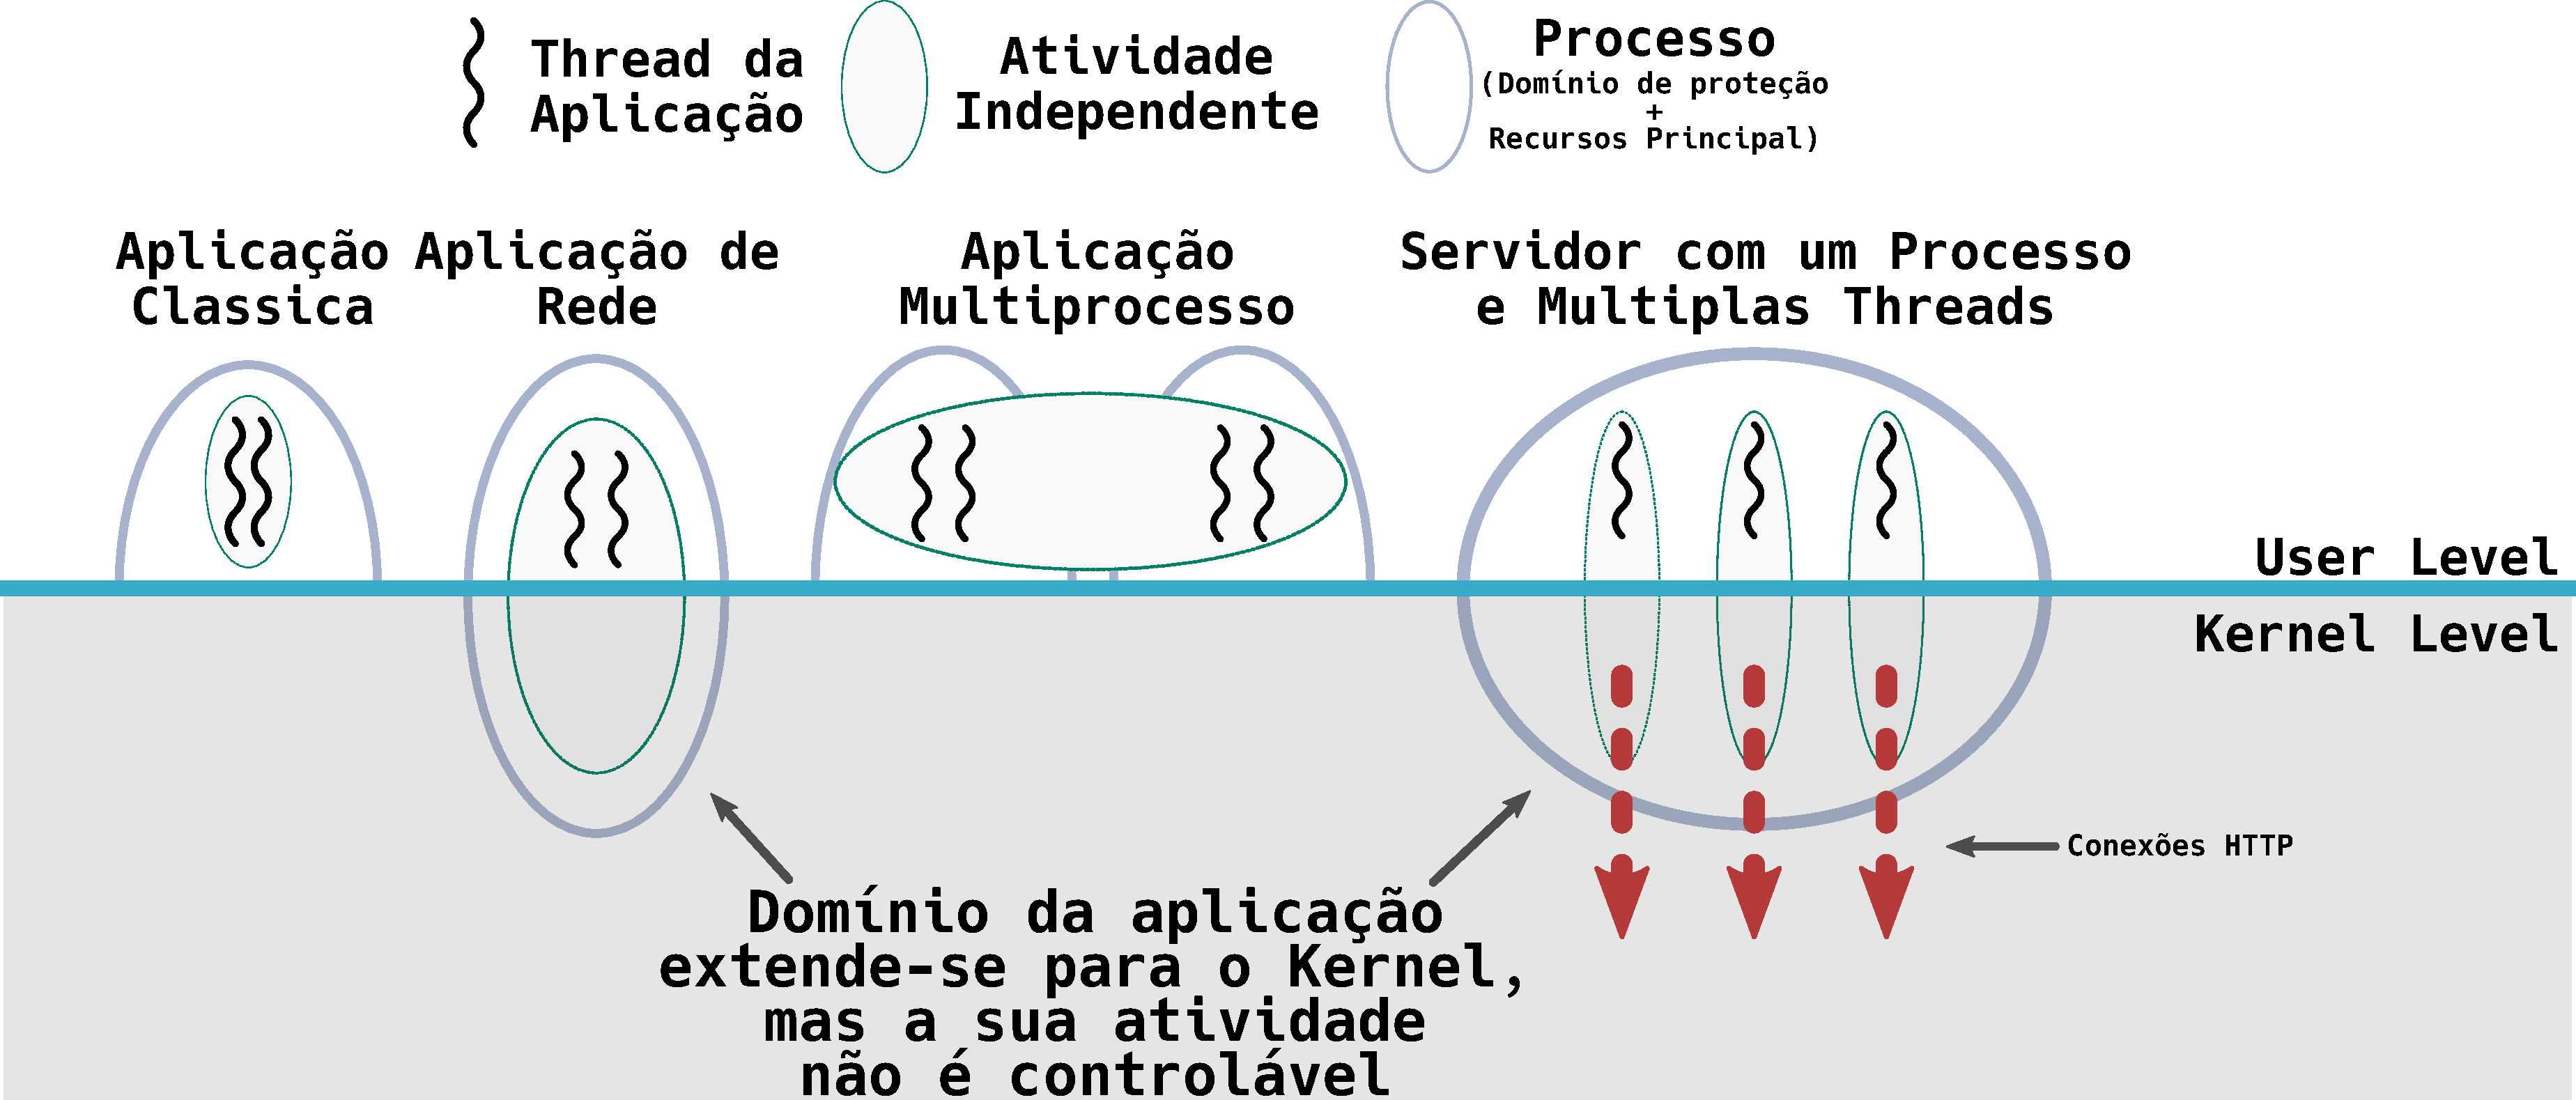
\includegraphics[width=\textwidth]{resource_constainer_scenarios} 
  \caption{Cenários das aplicações}
  \label{fig:resource_constainer_scenarios}
\end{figure}

Para ilustrar as questões referentes a gestão de recursos nos SOs, a Figura
\ref{fig:resource_constainer_scenarios} ilustra 4 cenários diferentes. O
primeiro cenário consiste em uma aplicação rodando em \textit{user space} que
não necessita de qualquer recursos diretamente controlado pelo Kernel, por
tanto, a seu consumo de recursos não se estende para o Kernel. O segundo
cenário representa uma aplicação que precisa utilizar recursos do Kernel para
terminar alguma de suas tarefas (e.g., um software que usa recursos de rede),
note que parte da aplicação consome recursos dentro do \textit{user space};
contudo, a outra parte da aplicação expande para o Kernel. O terceiro cenário
mostra múltiplos processos cooperando para concluir uma tarefa sem precisar de
do Kernel. Por fim, tem uma aplicação com um único processo que dispõe de
múltiplas threads que além de utilizar recursos no \textit{user space} também
demandam recursos oriundos do Kernel. Repare como sistemas tradicionais tem
pouco ou nenhum controle sobre os recursos consumidos, veja que esses casos
podem levar o escalonador a fazer contagens imprecisas levando o mesmo a
comportar-se de forma inadequada.

Inspirados pela falta de uma separação clara do gerenciamento de recursos por
parte dos SOs, \cite{resourcecontainers} sugeriram a criação de uma nova
abstração chamada \emph{Resource Containers (RC)}. Este é uma entidade que
logicamente contém todos os recursos utilizados pela aplicação para completar
uma determinada atividade. Seus atributos são usados para fornecer parâmetros
de escalonamento, limites de recursos, e \emph{QoS} para rede. A ideia é que o
Kernel cuidadosamente manipule esses recursos tal qual CPU e memória consumido
por um RC. O escalonador pode acessar as informações provenientes dos RCs e
utilizar elas para melhorar o processo de escalonamento.

A adição do RC cria uma clara distinção entre o domínio da proteção e o de
recursos, além de fornecer um controle fino sobre os recursos. O RC fornece um
mecanismo para ligar os recursos a uma thread, isto pode ser feito de forma
dinâmica e sob controle da aplicação (isto também é chamado de \emph{resource
binding}). Note que isto permite que múltiplas threads sejam associadas a
inúmeros RC ao mesmo tempo, mas por padrão, uma thread começa com um RC herdado
do processo pai. A aplicação poder religar-se para qualquer outro RC caso
exista a necessidade.

Uma das implicações diretas do RC é que uma aplicação associe informações com
uma atividade ao invés de associar a uma thread ou processo, isto permite que
o \emph{scheduler} forneça informações diretas para a atividade.

% TODO: Voltar no artigo e elaborar mais essa questão dos atributos
A alocação de atributos está diretamente associada com um modelo de
escalonamento relacionada com cada RC em um sistema. Uma thread é normalmente
escalonada de acordo com os atributos do RC na qual é limitada. Contudo,
se uma thread é multiplexada entre vários containers, pode custar muito o
reescalonamento, para cada mudança de binging. Na prática a thread deve ser
escalonada baseado na combinação entre alocação de recursos e uso de
RC. Para isto, o modelo define um \emph{scheduler binging} entre cada
thread e um conjunto de container sob o atual sendo multiplexado. 

É interessante observar que os containers formam hierarquias, ou seja, o uso de
um recurso usado por um container filho é restringido pelos parâmetros do
container pai. Por exemplo, se o container pai tem 70\% dos recursos
garantidos, então os container filhos não podem extrapolar esse limite.

De forma geral, para se utilizar o RC os autores sugerem uma API com as
seguintes características:

\begin{itemize}
	\item \textbf{Criar um Novo Container:} Por padrão, um container é criado
				como parte do \texttt{fork()} e são visíveis para a aplicação na forma
				de descritor de arquivos;
	\item \textbf{Ajuste do Container API:} Um processo pode mudar quem e o seu
				container pai;
	\item \textbf{Liberar o Container:} Um processo pode liberar a sua referência
				para um container usando o \texttt{close()};
	\item \textbf{Compartilhar Container entre Processos:} Quando um processo
				recebe uma referência para um container, ele pode usar o recurso como
				um \emph{resource context}. Isto permite mover uma aplicação ou
				computação entre vários domínios de proteção;
	\item \textbf{Atributos do Container:} Uma aplicação pode ler e ajustar
				atributos de um container;
	\item \textbf{Uso de Informações dos Containers}
	\item \textbf{Binding threads para um container:} Uma thread pode fazer o
				\emph{binding} para uma \emph{thread} a qualquer momento;
	\item \textbf{Restaurar o Scheduler Binding}
	\item \textbf{Binding de Socket ou Arquivo para um Container:} Um processo
				pode fazer o \emph{bind} de um socket ou arquivo para um container,
				assim o consumo subsequente dos recursos do kernel ficam no container.
\end{itemize}

\subsection{Nooks}
% deixar claro que tudo isso é no nível do kernel
\cite{nooks} conduziram uma pesquisa motivada pela busca por
adicionar mais confiabilidade e resiliência aos SOs de produção. O principal
problema que os autores buscam resolver são as constantes falhas geradas pela
expansão dos SOs por meio dos programas que controlam um dispositivo, também
conhecido com \emph{modules} ou \emph{device drivers} (Seção \ref{sec:dd}). O
artigo apresenta diversas evidências relacionadas as falhas geradas
pelas extensões feitas nos SOs e sugere uma nova abordagem chamada
\emph{Nooks}.

\emph{Nooks} é uma nova camada que se interpõe entre o Kernel e as extensões.
Essa camada comporta-se como um subsistema responsável por tratar as operações
passadas via kernel para os módulos e vice-versa; o controle feito sobre cada
parte representa uma camada a mais de verificação que adiciona mais segurança e
confiabilidade para o SO. Para fornecer a separação e controle dentro do SO, o
\emph{Nooks} apresenta o conceito de \emph{lightweight kernel protection
domain} (LKPD). Esta abstração permite isolar partes da memória no nível do
Kernel e atribuir diferentes permissões de leitura e escrita para a região.
Note que todo o controle entre as regiões de memória e a comunicação entre o
kernel com as extensões ocorre no domínio do kernel, não tendo relação direta
com o \emph{user space}.

O projeto do \emph{Nooks} foi totalmente guiado por dois princípios
fundamentais:

\begin{enumerate}
	\item \emph{Nooks} deve ser resistente a falhas e não tolerante a falhas;
	\item \emph{Nooks} deve ser projetado para evitar erros e não para evitar
				abusos.
\end{enumerate}

Esses dois princípios são importantes para deixar claro a área de atuação desta
técnica e para guiar os três objetivos principais que o \emph{Nooks} busca
atender:

\begin{enumerate}
	\item \textbf{Isolamento:} O \emph{Nooks} precisa ser capaz de isolar as
				extensões presentes no Kernel de forma a evitar falhas, consequentemente
				ele precisa ser capaz de detectar falhas antes que outras partes do
				SO sejam afetadas;
	\item \textbf{Recuperação:} A arquitetura precisa dar suporte para a
				recuperação da aplicação em caso de falhas;
	\item \textbf{Compatibilidade com versões anteriores:} \emph{Nooks} deve ser
				compatível com as extensões já existentes e usadas.
\end{enumerate}

\begin{figure}[!h]
  \centering
  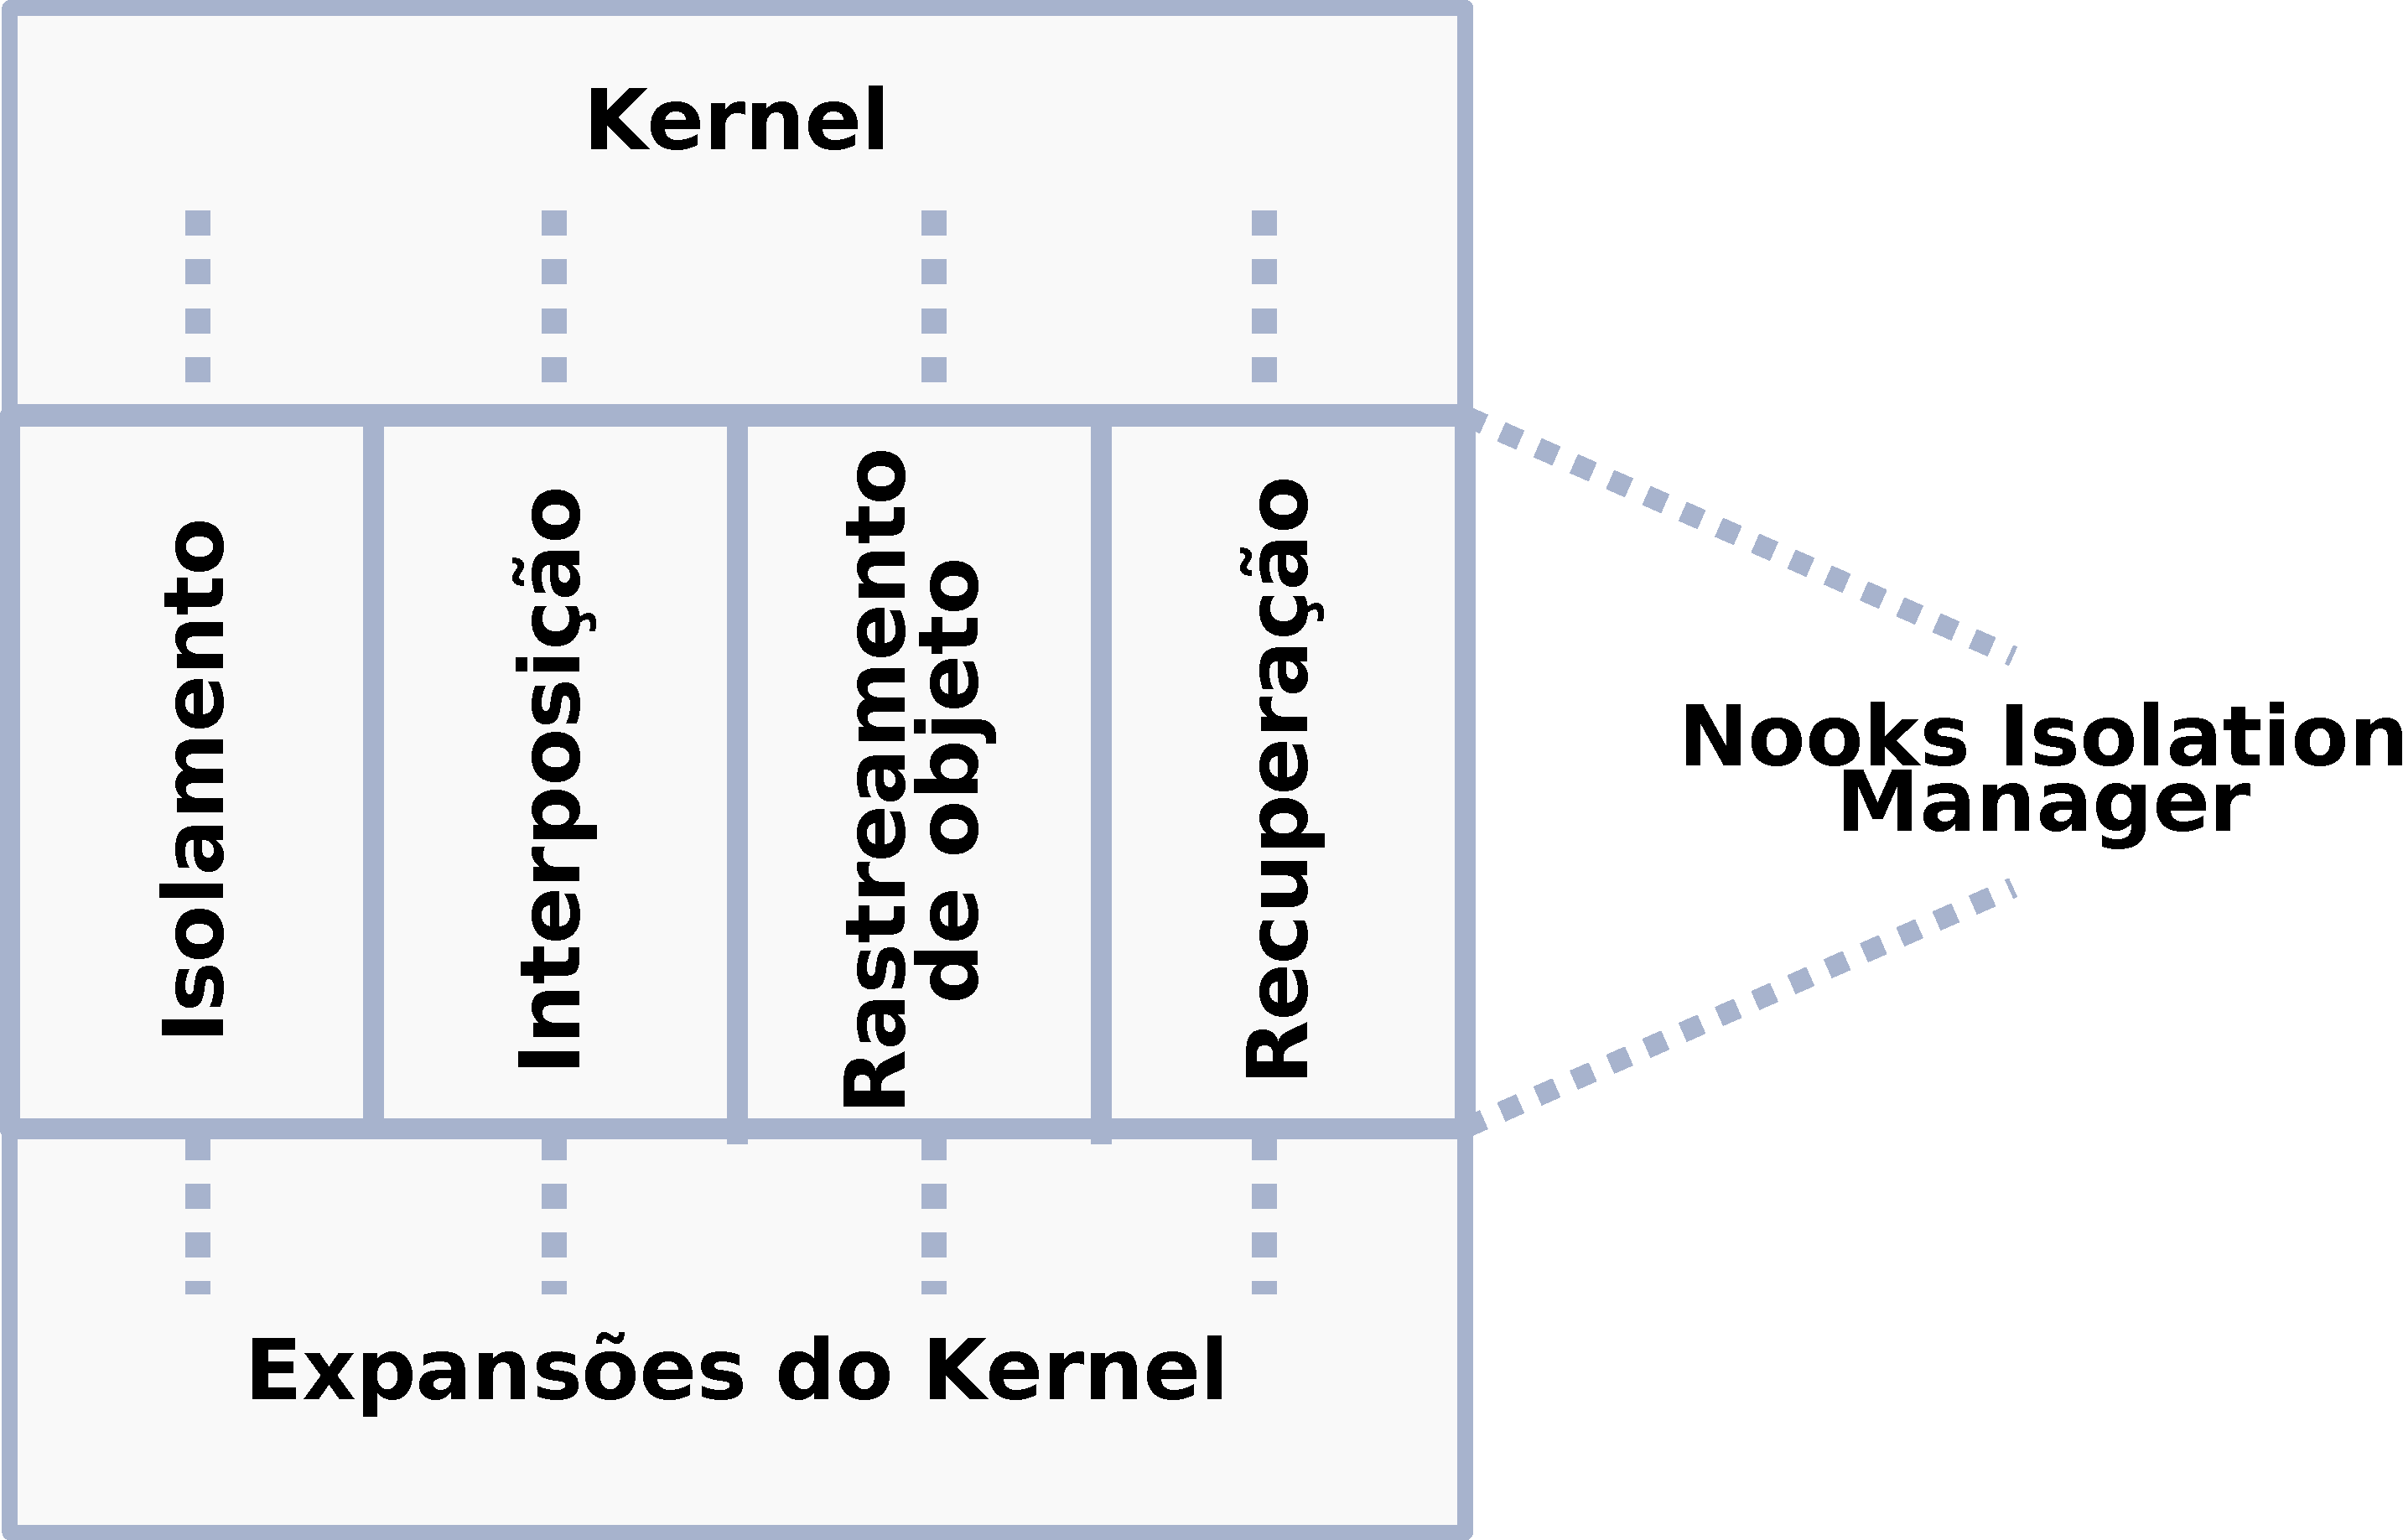
\includegraphics[width=0.8\textwidth]{nooks_nim}
  \caption{Visão geral da arquitetura do Nooks \citep{nooks}}
  \label{fig:nooks_nim}
\end{figure}

A Figura \ref{fig:nooks_nim} ilustra de forma geral a arquitetura do
\emph{Nooks}. Note que a comunicação entre o Kernel e as extensões (vice-versa)
precisam passar pelo \emph{Nooks}. Esse intermédio é conduzido pelo \emph{Nooks
Isolation Manager (NIM)} que é o responsável por implementar os objetivos do
projeto. O \emph{Nooks} precisa estender-se em parte para o Kernel e em parte
para as extensões. No Kernel, é preciso alterar aquelas funções que são
disponibilizadas para as extensões ou que interagem com os módulos. Felizmente,
este tipo de função pode ser detectada por algum padrão que por sua vez pode
ser abstraído para um \emph{script} e este tipo de modificação precisa ser
feita uma única vez. Do ponto de vista dos módulos, no geral, são poucos os
casos que precisam ser alterados diretamente uma vez que este faz uso dos
recursos fornecido pelo Kernel. Normalmente, módulos que exportam estruturas de
dados próprias e que são exportáveis para o Kernel, consequentemente precisam
ser alteradas.

O \emph{Nooks} fornece isolamento por meio do LKPD uma vez que toda extensão
adicionada ao SO executa dentro do seu próprio LKPD que por sua vez é chamado
de \emph{contexto de execução}. Os domínios utilizam o mesmo nível de proteção
fornecido pelo processador para o Kernel, com a diferença de que o acesso de
escrita para certas porções é limitada e gerenciada pelo \emph{NIM}. Neste
sentido, podemos dividir o esquema de isolamento do \emph{Nooks} em duas partes:
o gerenciador de memória e o \emph{Extension Procedure Call} (XPC).

\begin{figure}[!h]
  \centering
  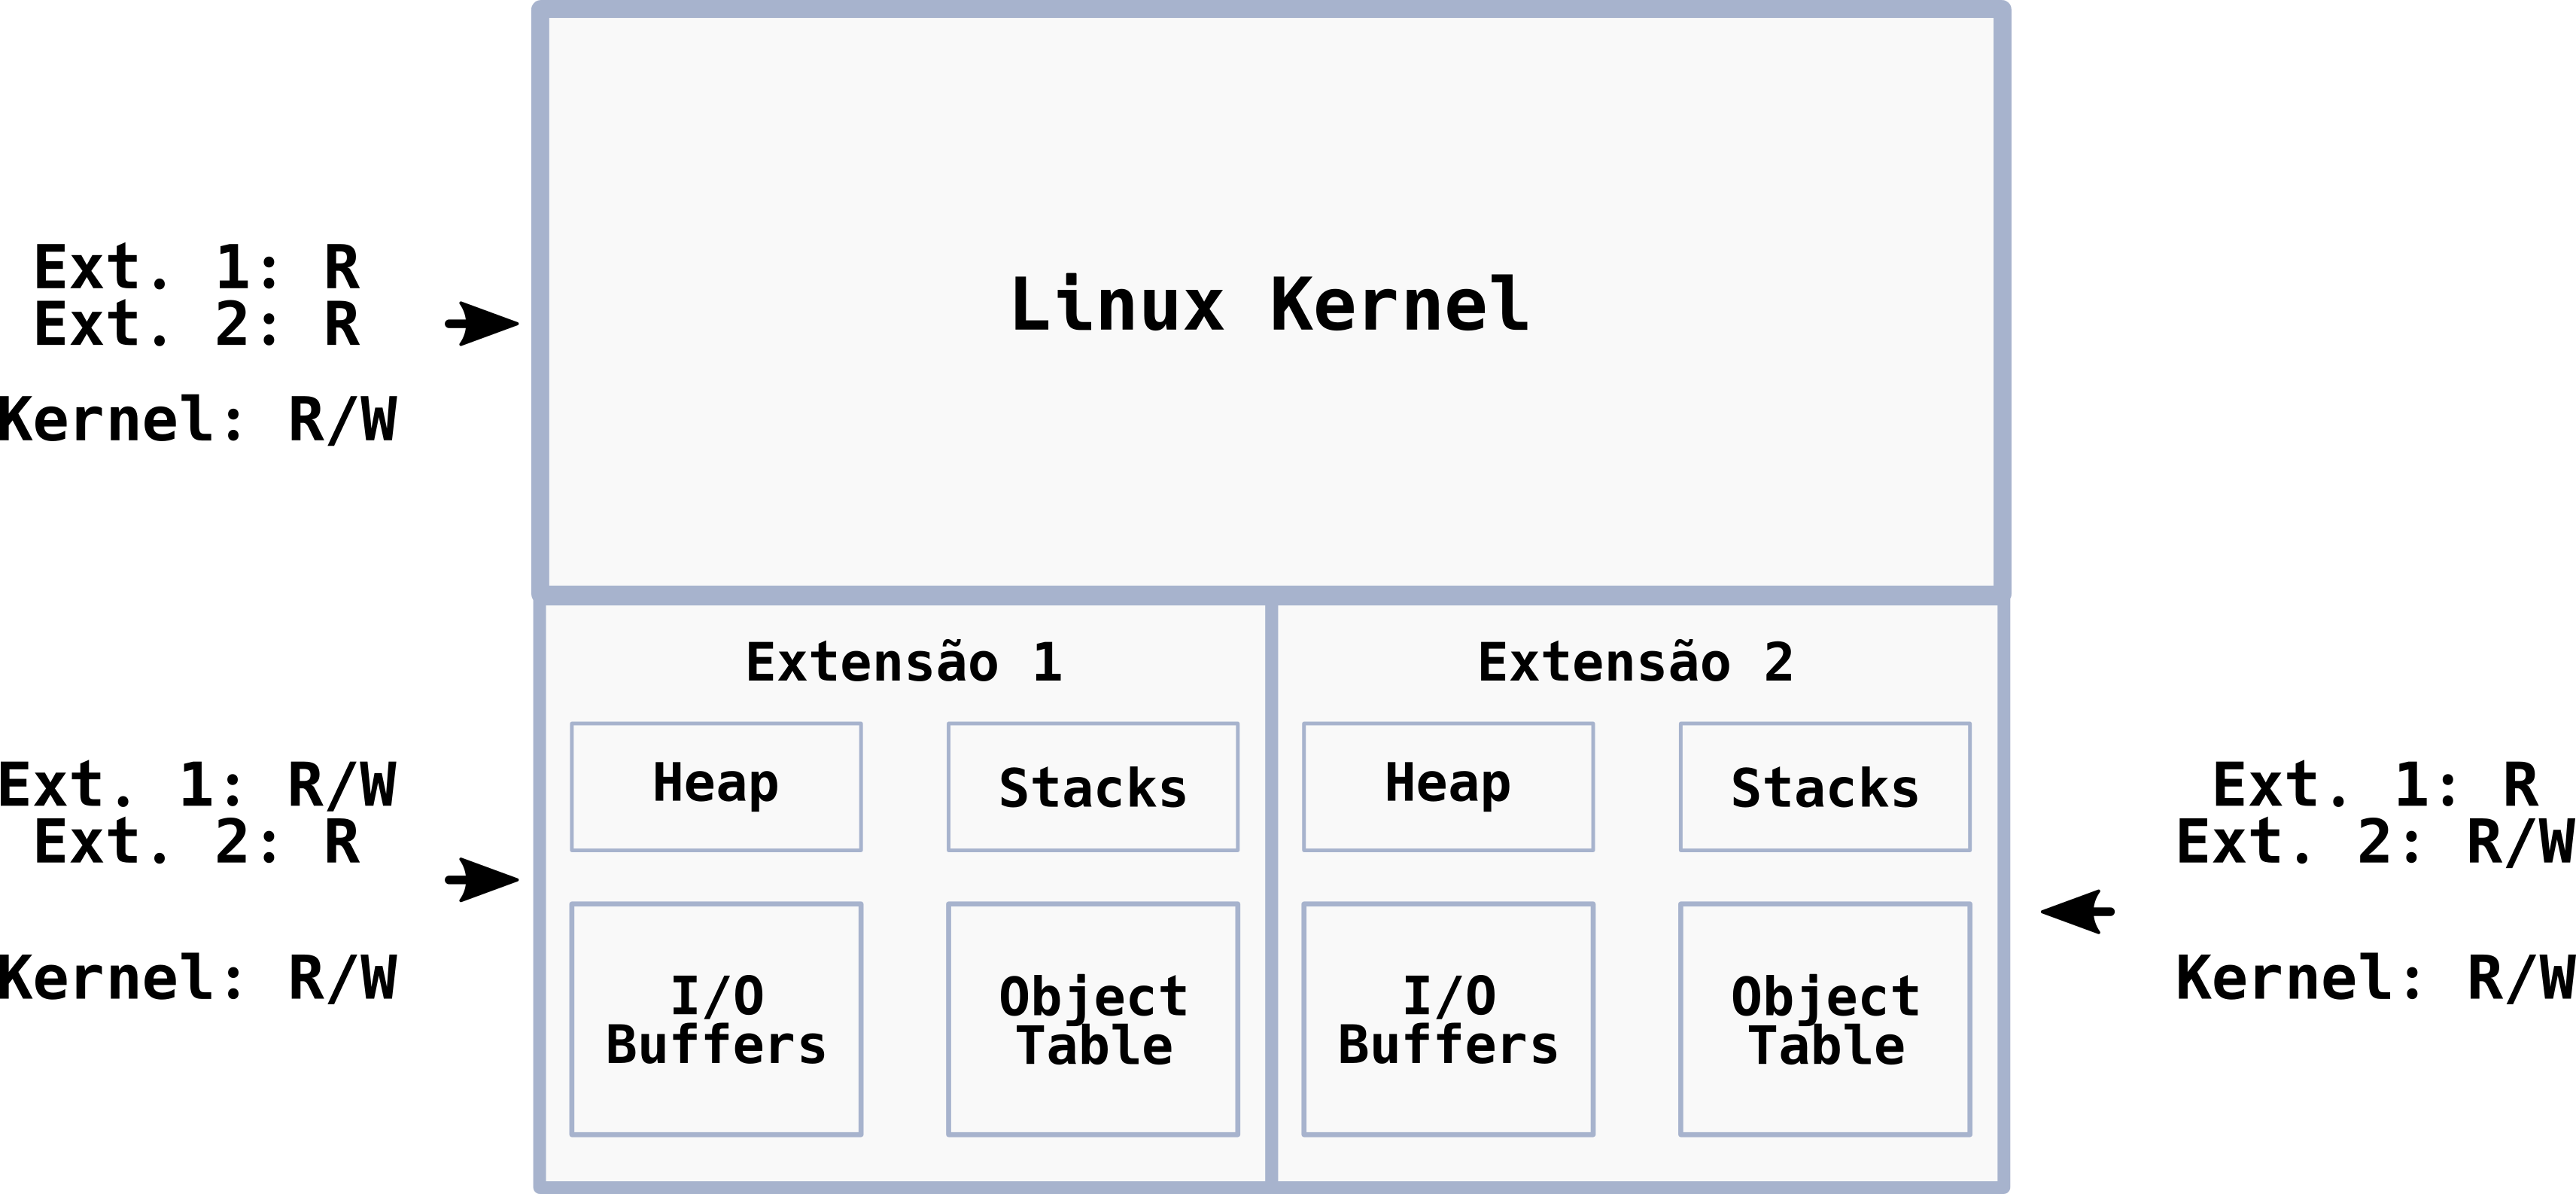
\includegraphics[width=0.8\textwidth]{nooks_mem}
  \caption{Acesso a memória do Nooks \citep{nooks}}
  \label{fig:nooks_mem}
\end{figure}

O gerenciador de memória do \emph{Nooks} é responsável por alocar, desalocar e
manipular os LKPD. A Figura \ref{fig:nooks_mem} ilustra o \textit{kernel
address space}, note que o Kernel tem permissão de escrita e leitura sobre toda
a memória, mas os LKPD mostrados só tem acesso de leitura e escrita a si mesmo.
A leitura de outras regiões de memória de dentro de um LKPD depende do controle
de acesso feito pelo NIM, mas no geral só é permitido a leitura de outras
regiões da memória.

O outro mecanismo de isolamento fornecido pelo \emph{Nooks} é o XPC, este atua
como um serviço de transferência de controle criado para isolar as operações
feitas dentro do Kernel. A transferência de controle pode acontecer em duas
vias: do Kernel para a extensão (\texttt{nooks\_driver\_call}) e da extensão
para o Kernel (\texttt{nooks\_kernel\_call}). Basicamente essas funções esperam
três argumentos: um ponteiro para a função que será executada, uma lista de
argumentos e o domínio em que será executada. Toda vez que a rotina de
transferência é chamada o contexto da stack que realizou a chamada é salva e o
\emph{Page Table} para o novo domínio alvo carregado.

Um dos objetivos do \emph{Nooks} é o de ser usado em SO de produção, para isto
ele tem uma de se integrar com o SO de forma a causar o menor impacto possível
nas extensões. Por isto, o \emph{Nooks} isola as extensões com o XPC e também
implementa um mecanismo de rastreamento de estruturas de dados chamado
\emph{object-tracking} (parte do \emph{NIM}). O \emph{object-tracking} tem três
recursos básicos: manter uma lista de estruturas de dados do Kernel que são
manipulados por uma extensão, controlar todas as modificações para estas
extensões e fornecer informações de objetos para limpeza de dados quando a
extensão falhar. O rastreamento dos objetos começa com o armazenamento de todos
os objetos em uso por uma extensão e em seguida é feita uma associação entre o
Kernel e as versões das extensões.

Por fim, o \emph{Nooks} possuí um mecanismo de recuperação que busca detectar
falhas de software quando uma extensão é chamada de forma inapropriada ou se
uma extensão está consumindo muitos recursos. A estratégia de recuperação é
subdividida em duas partes: \emph{recovery management} e \emph{user-mode
agent}. O primeiro é responsável por desalocar recursos e se necessário
realocar novamente os mesmos. O segundo é quem coordena a ação de recuperação e
é definida no espaço de usuário. Note que a flexibilidade do \emph{agent-mode}
permite várias possíveis formas de recuperação, sendo a mais direta forçar a
remoção da extensão, seguida da reinserção e em seguida prosseguindo com a
execução da aplicação.

O \emph{Nooks} utilizou uma base de dados de inserção de falhas em módulos para
validar a sua eficácia, conseguindo tratar 99\% dos casos. Além disto, os
autores também validaram o trabalho da perspectiva do desempenho e notaram que
na maioria dos casos os gastos com a estrutura são compensado pelas vantagens.

\subsection{Mondrian Memory Protection e Mondrix}

\cite{mmp} buscaram explorar técnicas para realizar controle fino sobre da
memória, com o objetivo de adicionar mais confiabilidade e segurança para os
SOs. Os autores discutem os problemas associados com a decisão de se promover
isolamento por meio da separação do espaço de endereçamento dos processos, que
por sua vez faz com que todas as \emph{threads} de um processo compartilhem um
mesmo domínio de proteção. Além disto o modelo de paginação adotado impõe um
tamanho fixado, logo, o menor compartilhamento possível é o de uma página que
tem o mesmo nível de permissão para todos os elementos contido nela. Os autores
argumentam que apesar das vantagem oferecidas pelo modelo atual, muitos
problemas de segurança e estabilidade do sistema são comprometidos. Dois
exemplos são apontados pelos autores, o primeiro ilustra o caso do Servido
Apache que pode carregar vários \textit{plugins} externos, contudo, se algum
código malicioso ou defeituoso for carregado este comprometerá toda a
estabilidade do servidor (em alguns casos quebrando a aplicação). Outro exemplo
refere-se ao acesso de ponteiros em outros domínios da memória (por exemplo,
acesso do espaço de usuário para o do Kernel) que atualmente não são permitidos
sendo necessário realizar operações de cópias.

% TODO: Figura Y

Os autores defendem que mecanismos de controle fino do acesso à memória podem
trazer grandes benefícios em termos de segurança, confiabilidade e em certos
casos ganho de desempenho. Nesse sentido \cite{mmp} propuseram uma abordagem
que permite o controle de acesso da memória no nível do tamanho das palavras de
dado, para isto é apresentando um novo tipo de abordagem baseada em hardware e
software chamada de \emph{Mondrian Memory Protection (MMP)}~\citep{mmp}. Além
disto uma implementação prática chamada de \emph{Mondrix}~\cite{mondrix} foi
feita no GNU/Linux. A Figura Y, resume a representação de memória que o MMP
busca atingir, repare que não existem porções de memória específica; note que a
memória é dividida em diversos compartimentos chamados de \emph{Protection
Domain (PD)}. Um PD é definido como um contexto que determina a permissão para
executar um código. Cada PD é independente do espaço de endereçamento; cada PD
pode conter múltiplas threads, mas cada thread só pode pertencer a um único PD.
O projeto do MMP é guiado por três requisitos:

\begin{enumerate}
	\item \textbf{Diferente}: Cada PD diferente pode ter um domínio distinto
				para a mesma região de memória;
	\item \textbf{Pequeno}: A granularidade de compartilhamento deve ser menor
				do que uma página;
	\item \textbf{Revogável}: Um PD é dono da sua própria região de memória e
				pode mudar a forma como outros domínios veem a sua memória.
\end{enumerate}

% TODO: FIGURA K
% TODO: FALAR DA SEGMENTAÇÃO NA FUNDAMENTAÇÃO
Os autores afirmam que o MMP tem a semântica da segmentação sem os problemas. O
MMP fornece controle fino sobre a proteção dos dados compartilhados, utiliza
endereçamento linear, é compatível com a \emph{ISA} existentes, não necessita de
registradores de segmentos, possui um mecanismo simples de revogação de
permissões e não tem ponteiros marcados. A Figura K mostra o comparativo entre
a abordagem utilizando segmentos e o MMP. Para que o MMP possa garantir o
controle de acesso à memória este precisa verificar as permissões de acesso
feitas por cada operação de \emph{load/store}, isto claramente consome mais
recursos computacionais. Por isto o MMP é uma solução que também depende da
utilização de um hardware personalizado.

% TODO: FIGURA G

A Figura G ilustra a arquitetura de hardware proposta para a implementação do
MMP, note que ela introduz muitos elementos novos. %TODO: Descrever o hardware

Da perspectiva do Software, o Mondrix \citep{mondrix} sugere a utilização de um
novo elemento chamado de Supervisor de Memória, este é dividido em duas partes:
parte superior responsável pelo controle do acesso; parte inferior responsável
por escrever nas tabelas de permissão. A parte superior é a mais importante,
sendo responsável por manter e controlar as políticas, interface com o Kernel,
rastrear objetos compartilhados e implementar grupos de permissão. As
definições de permissão da memória é descrita por três elementos:

\begin{enumerate}
	\item \emph{Permissão de Acesso}: As permissões de acesso são definidas pelo
				seguinte conjunto de elementos: permissão do domínio, \emph{gates},
        tabela de \emph{stack};
	\item \emph{Dono da Memória}: Define quem tem autoridade sobre a região de
				memória (domínio). Note que o espaço de endereçamento é contínuo e sem
				sobreposição, logo, cada região tem apenas um dono;
	\item \emph{Permissões Exportadas}: É possível exportar as permissões de
				acesso, isto é feito para permitir que outras regiões chamem códigos
				fora do seu domínio. Contudo a exportação pode ser controlada de forma
				que outros trechos que acessem o código, tenham uma visão limitada da
				região.
\end{enumerate}

Dado esses elementos, o Supervisor de memória atual tomando as decisões
referentes ao acesso a uma dada região da memória.

Um aspecto interessante de se notar do Supervisor de Memória é a sua separação
lógica do alocador de memória. O Mondrix permite que o Kernel escolha qual
alocador de memória deseja utilizar, isto é possível pois um domínio solicita
memória para o alocador e o Supervisor só estabelece as permissões para a
memória solicitada.
% Gosto muito dessa ideia de separar o alocador do controlador de acesso à
% memória, na minha opinião em termos práticas essa é uma das ideias mais
% valiosas desse trabalho.

O Supervisor também é responsável por revogar permissões quando uma região de
memória é liberada, além de manter o rastreamento de qual domínio tem acesso a
qual região de memória. O Supervisor também gerência o acesso a \emph{stack}
das \emph{threads} (uma \emph{thread} só pode controlar \emph{stacks} que estão
no seu domínio), cria e destrói proteções de domínio e também valida as
políticas de acesso.

\subsection{SpaceJMP}
\label{sec:mvas}

Toda vez que um processo é criado, ele inicializa diferentes estruturas de
dados relacionadas a sua execução. Um dos elementos fundamentais dos processos
é o espaço de endereçamento virtual (\emph{Virtual Address Space - VAS}), que é
completamente acoplado aos processos. Normalmente, as VAS são maiores que a
memória física e são totalmente isoladas de outros processos. Se um processo
precisar compartilhar dados com outros processos, será necessário criar e
gerenciar uma região da memória que permita que outros processos leia e/ou
escrevam na área compartilhada. O atual modelo de VAS não da suporte para
passar estruturas de dados baseadas em ponteiros entre processos, normalmente,
é necessário serializar os dados para que tal tarefa seja possível; esses
mecanismos tem se tornado um incomodo.

\begin{figure}[!h]
  \centering
  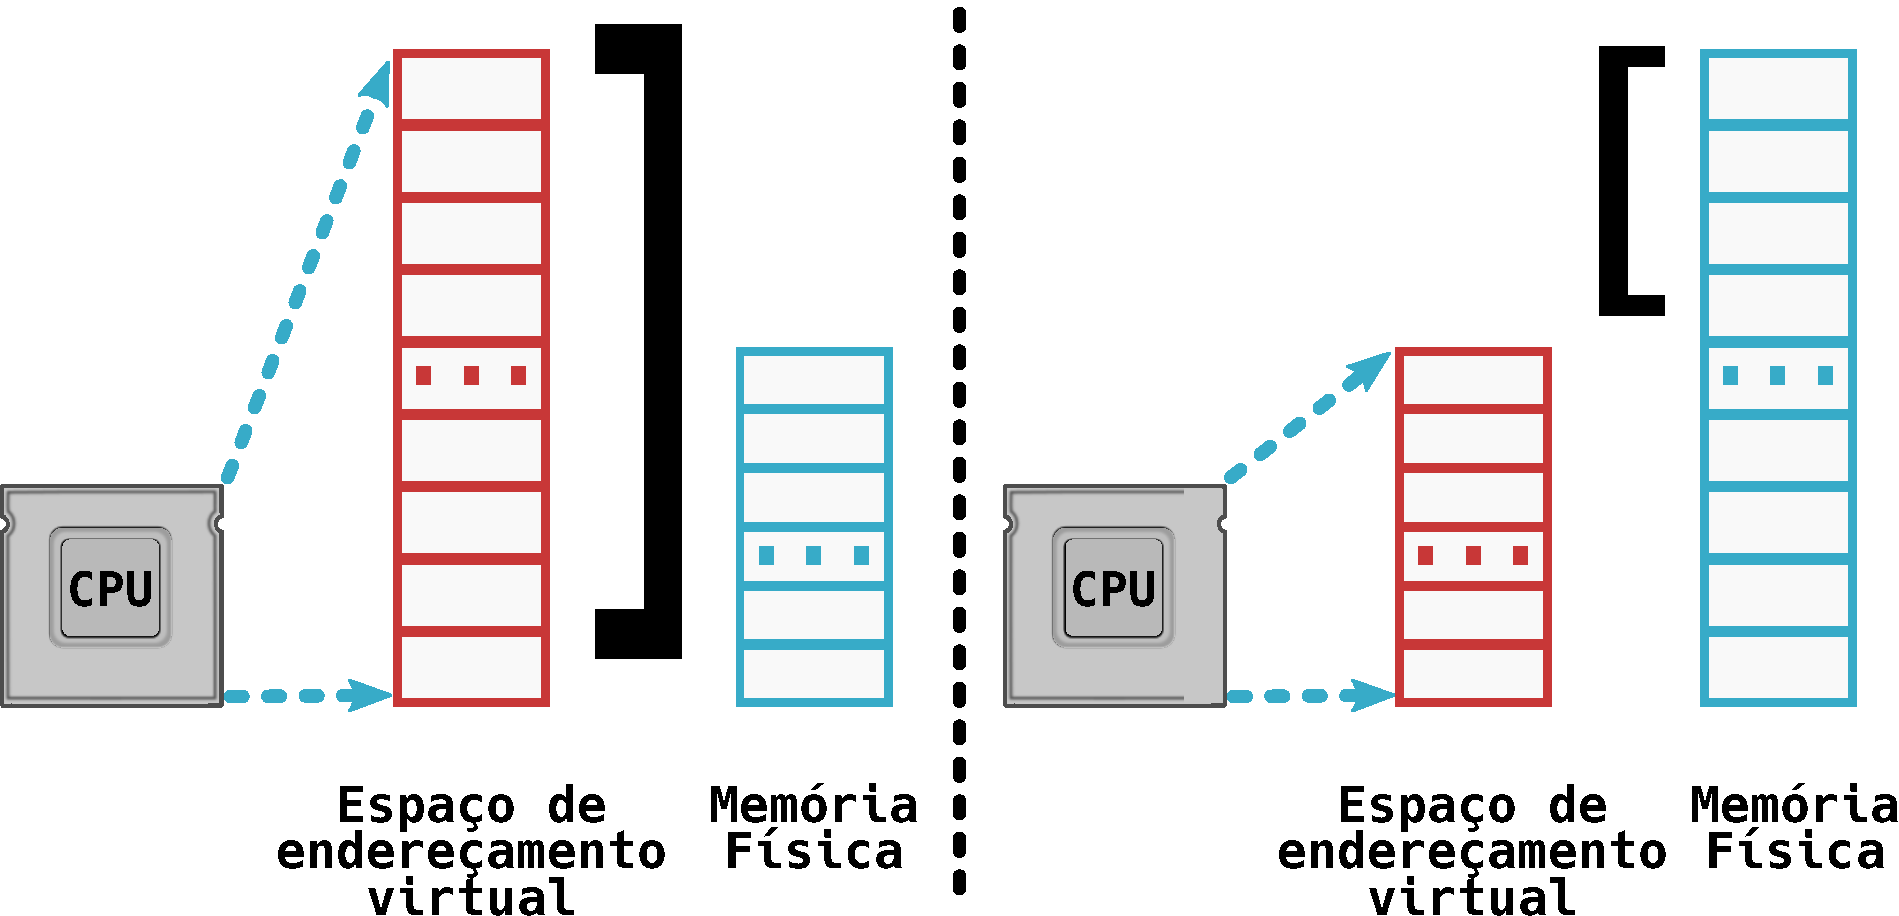
\includegraphics[width=.7\textwidth]{vas_vs_physical_address} 
  \caption{VAS e Memóra Física}
  \label{fig:vas_vs_physical} 
\end{figure}

Em 1990s, os processadores tinham poucos bits para o VAS, mas eram o suficiente
para endereçar toda a memória física disponível na época. Apesar disto, durante
esse período, o tamanho da memória cresceu consideravelmente e os processadores
não foram capaz de endereçar diretamente todo o endereço de memória disponível
\cite{crowley}. A Figura \ref{fig:vas_vs_physical} exemplifica o problema
mencionados acima; a parte da esquerda ilustra uma CPU com bits suficientes
para a VAS de forma que consegue endereçar todo o espaço de endereçamento
físico da memória. O lado direito da figura representa uma situação na qual a
VAS é menor do que a memória física, assim, um um único processo não é capaz de
acessar toda a memória física disponível; isto impõe um limite ao processo
quanto ao tamanho que este pode ter. A situação na Figura
\ref{fig:vas_vs_physical} não é uma novidade, enquanto a industria não produzia
novos processadores com bits extras para elevar o tamanho da VAS, os
desenvolvedores tiveram que utilizar de vários artifícios para superar o
problema de bits insuficientes. Hoje em dia, este problema está sob controle
uma vez que os processadores atuais possuem um grande espaço de endereçamento.
Contudo, estamos no inicio de uma geração conhecida por \emph{data-centric} na
qual será dominada por grandes memórias não-voláteis \citep{outlook}, assim,
simplesmente incrementar o total de bits para a VAS nas CPUs não vai funcionar.
Elevar o número de bits na VAS tem impactos na produção, desempenho e consumo
de energia \citep{spacejmp}.

Um dos problemas do modelo de processos atuais está relacionado a representação
de como estruturas de dados baseadas em ponteiros fora dos limites dos
processos. A serialização de dados ou ponteiros especiais podem ser empregados
para resolver este problema, contudo, ambos os métodos são um incomodo,
ineficiente e em muitos casos confusos \cite{spacejmp}. O segundo problema está
associado com a tarefa de coordenar o compartilhamento de memória entre
vários processos, uma vez que está é uma tarefa complicada e tediosa.

Para tentar resolver os problemas citados, \cite{spacejmp} propuseram uma
técnica chamada \emph{SpaceJMP}. Os autores propõem desacoplar a VAS dos
processos e permitir que um único processo tenha Múltiplas VAS (MVAS)
associadas a si. Nesse contexto, a VAS é promovida para um objeto de
primeira-classe no SO e da ao processo a habilidade de gerir as muitas
VAS.

\begin{figure}[!h]
  \centering
  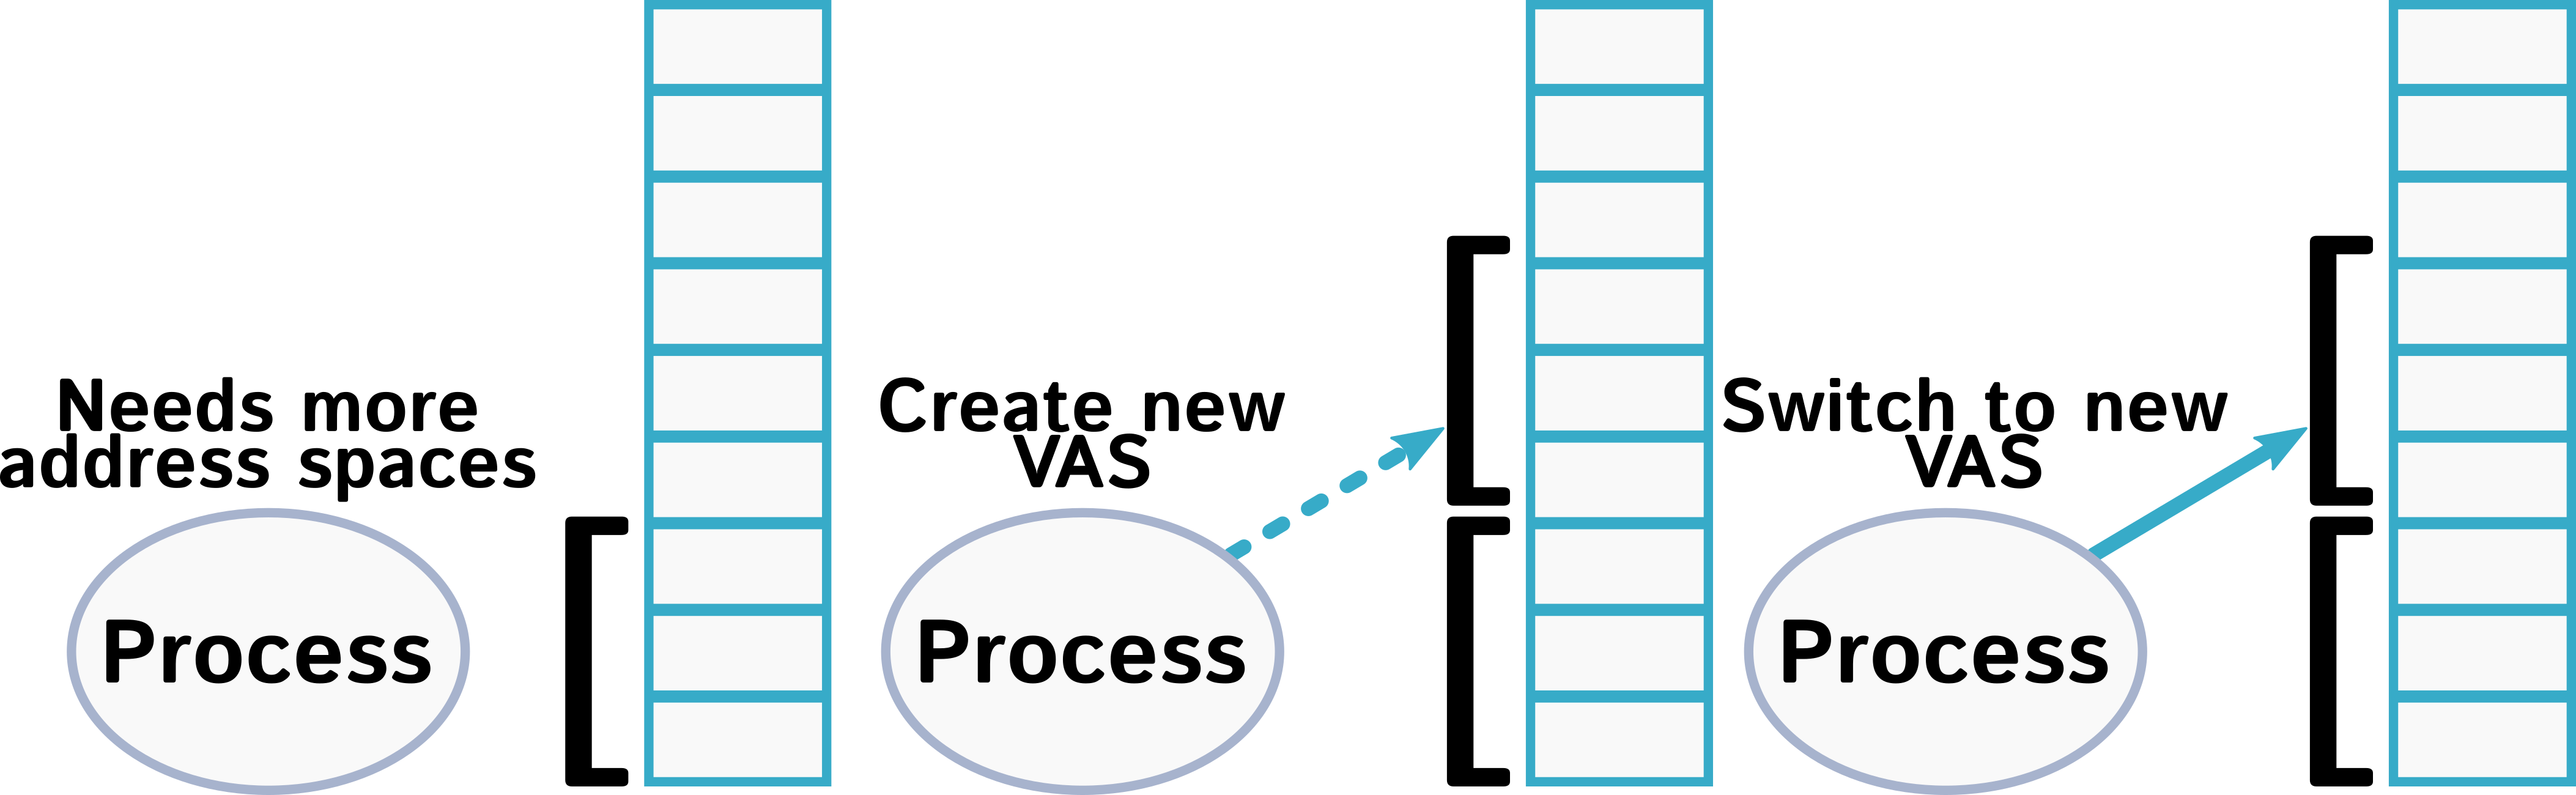
\includegraphics[width=.7\textwidth]{solve_huge_address_memory}
  \caption{Resolvendo o problema de endereçar memórias físicas grandes}
  \label{fig:large_memory}
\end{figure}

A Figura \ref{fig:large_memory} ilustra como MVAS resolver o problema de
endereçar memórias físicas maiores do que o VAS. Basicamente, todo processo
pode criar multiplas VAS e mudar entre elas. Se os processos precisarem de mais
memória do que o disponivel, basta criar um novo address pace com o começo
apontando para uma região de memória não utilizada e em seguida anexar a nova
VAS ao processo. Com isto, torna-se possível que o processo faça trocas entre
as diferentes VAS. O problema da serialização e compartilhamento de dados podem
ser simplificados pela MVAS uma vez que está pode criar uma VAS e permitir que
multiplos processos se anexem à ela.

\begin{figure}[!h]
  \centering
  \includegraphics[width=.7\textwidth]{traditional_vs_mvas} 
  \caption{VAS e MVAS \citep{spacejmp}}
  \label{fig:traditional_vs_mvas} 
\end{figure}

A Figura \ref{fig:traditional_vs_mvas}, ilustra a principal diferença entre um
processo com uma VAS acoplada para um modelo na qual a VAS é desacoplada
(MVAS). O lado esquerdo da Figura mostra um processo tradicional como explicado
na Seção \ref{sec:processos-e-threads}. O lado direito da figura, representa um
processo com múltiplas VAS e diferentes informações dentro de cada \emph{Heap}
e segmentos de memória. Nesse novo cenário, a pilha, os dados, e os segmentos
de texto são compartilhados entre as múltiplas MVAS. Por fim, é importante
notar que os processos precisam manter a informação sobre a atual VAS em
execução.
 
Os autores da técnica fizeram uma implementação para GNU/Linux. A principal
funcionalidade do MVAS foi exposta para o usuário via \emph{system calls}. A
lista a seguir mostra o conjunto de funções expostas para o usuário:

\begin{itemize}
  \item \texttt{vas\_create()}: Cria uma nova VAS com o nome indicado;
  \item \texttt{vas\_delete()}: Remove uma VAS criada previamente;
  \item \texttt{vas\_find()}: Encontra uma VAS de acordo com o nome;
  \item \texttt{vas\_attach()}: Anexa uma VAS ao processo;
  \item \texttt{vas\_detach()}: Desanexa uma VAS do processo;
  \item \texttt{vas\_switch()}: Muda a atual VAS instalada no processo para outra.
\end{itemize}

\begin{figure}[!h]
  \centering
  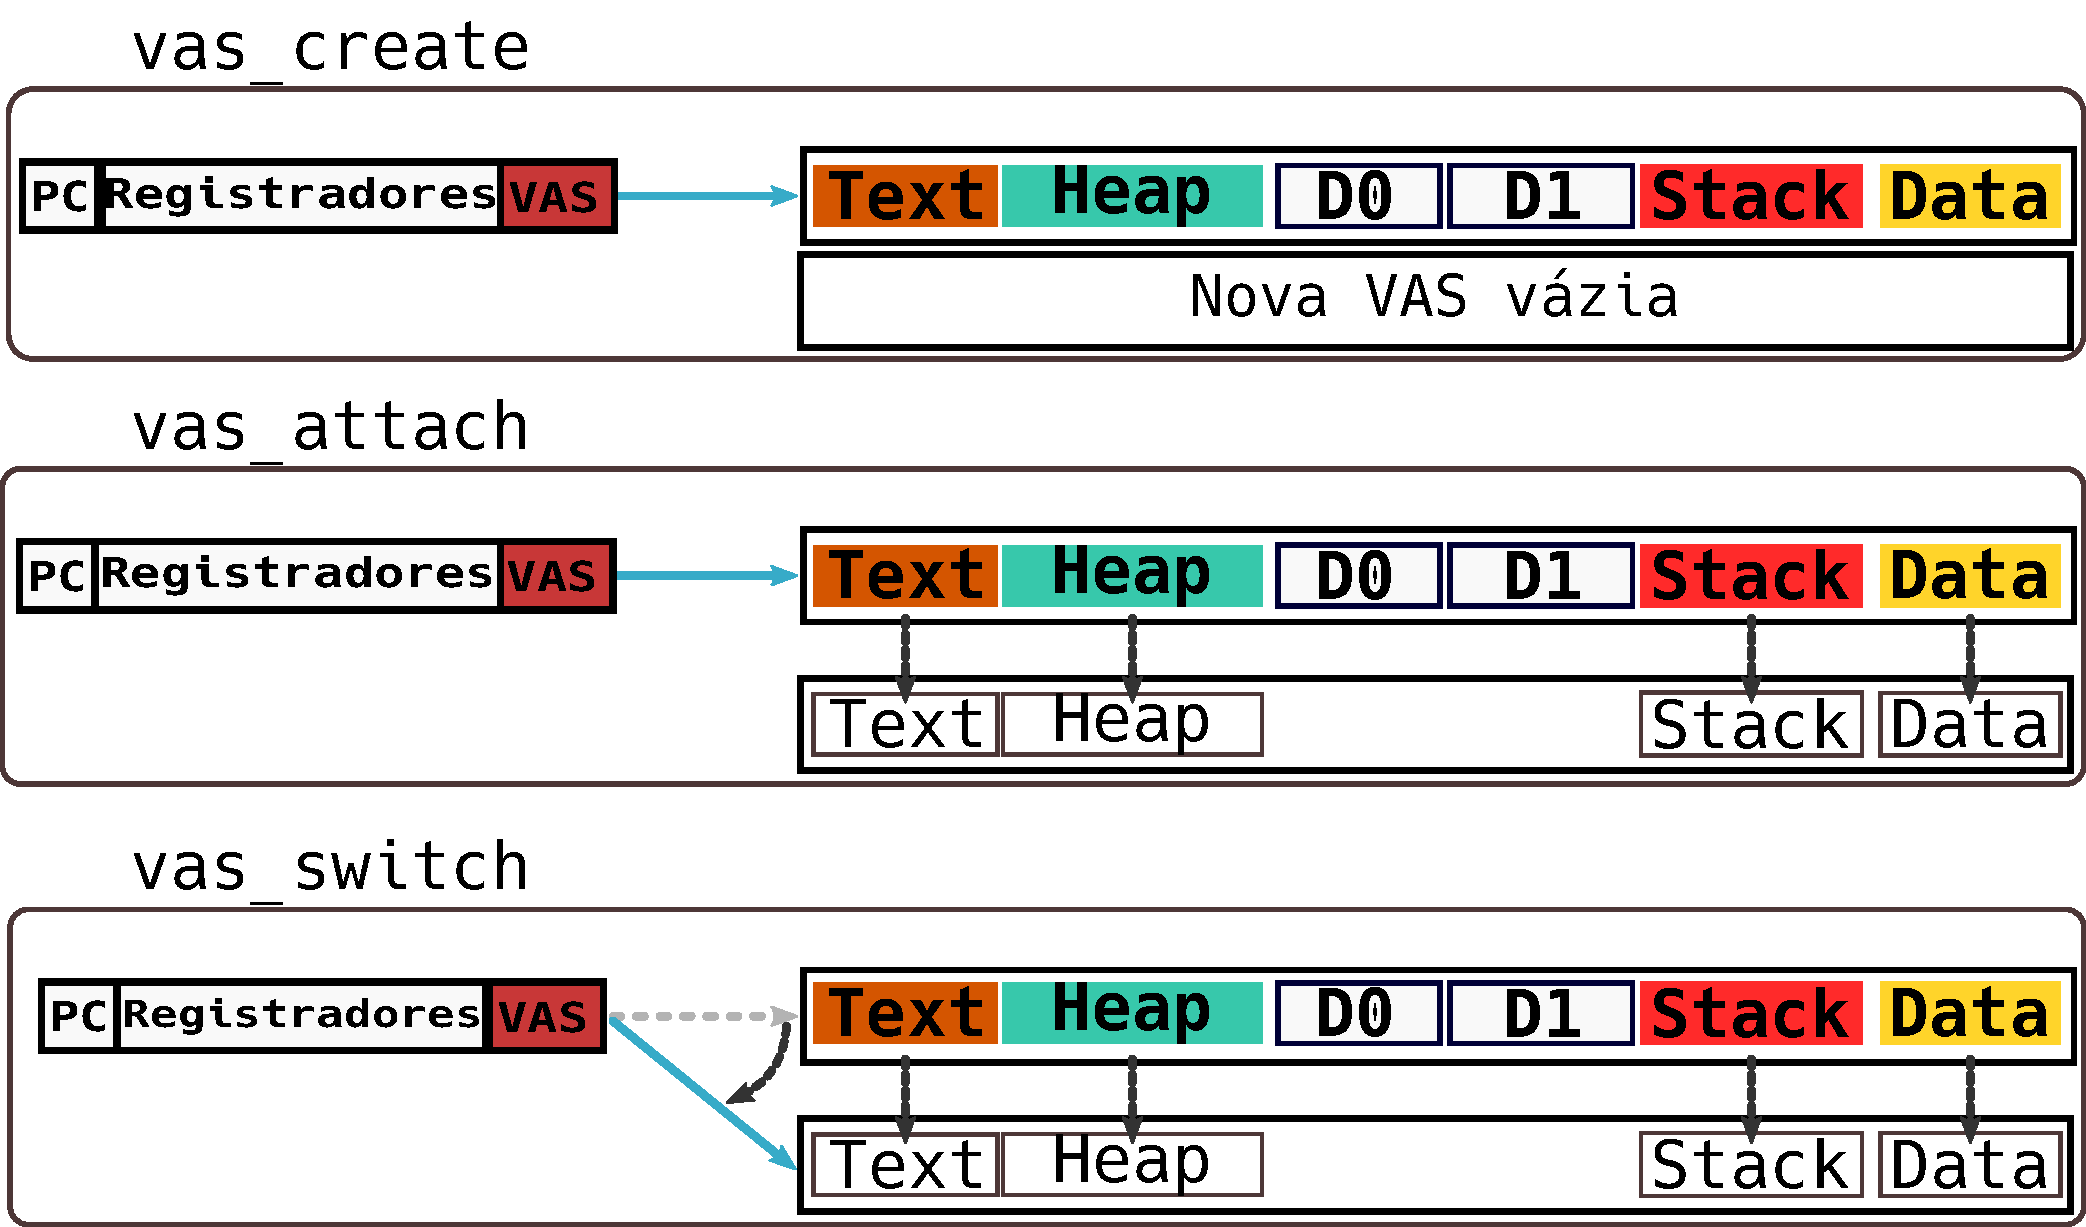
\includegraphics[width=.7\textwidth]{mvas_example} 
  \caption{System Call disponibilizada pelo SpaceJMP \cite{ellarge}}
  \label{fig:mvas_example}
\end{figure}

A Figura \ref{fig:mvas_example}, ilustra o comportamento da chamada de sistemas
implementadas. O topo da figura mostra um processo normal com uma VAS padrão
associada a si; em seguida a chamada para a função \texttt{vas\_create()} é
feita de forma a criar uma nova VAS. Após criar, é preciso anexar a VAS ao
processo por meio da chamada de sistema \texttt{vas\_attach()}, por fim, o
processo pode mudar entre as VAS por meio da chamada para
\texttt{vas\_switch()}.

\subsection{Light-weight Contexts}

O fluxo de execução do processo é controlado pelo \textit{Program Counter (PC)}
juntamente com os dados da memória, por sua vez, o escalonador é a entidade que
orquestra quando tirar e inserir um novo processo na CPU. Consequentemente,
tanto o PC quando os demais dados do processo são mantidos juntos no nível do
kernel.

\cite{litton} afirmam que o desacoplamento do isolamento da memória, estado de
execução e separação dos privilégios dos processos trazem benefícios. Com tal
ideia em mente, os atores sugerem uma nova abstração de processos chamada de
\textit{lightweight-context (lwc)}. Basicamente, cada processo pode ter um
(lwC root) ou mais lwCs na qual cada um contém o seu próprio mapeamento
virtual da memória, descritor de arquivos e credenciais. Opcionalmente, a API
do lwC permite controlar quais elementos podem ser compartilháveis ou não entre
os lwCs.

Um lwC compreende um mapeamento de memória virtual, uma coleção de mapeamento
de páginas, \emph{bindings} de descritores de arquivos e conjuntos de
credenciais; sempre que um novo processo é criado, o sistema cria um novo lwC
para ele. A aplicação pode acessar todas as funcionalidades do lwC via espaço
do usuário através de chamadas de sistemas que fazem o controle fino dos
comportamentos fornecidos.  As chamadas mais interessantes são:
\texttt{lwCreate()} e \texttt{lwSwitch()}. O \texttt{lwCreate()} tem uma
semântica similar ao \texttt{fork()}: depois que o \texttt{lwCreate()} retorna,
o atual processo tem um novo lwC (filho) associado consigo mesmo que consiste
em um \emph{snapshot} do processo que foi chamado. Esse \emph{snapshot} se
difere do \texttt{fork()} uma vez que nenhum PID novo ou thread é criado.
Depois da criação do processo filho, a aplicação é livre para fazer a troca
(com o \texttt{lwSwitch()}) para algum de seus \emph{snapshots} a qualquer
momento.

A Figura \ref{fig:lwc} ilustra a operação de troca entre diferentes lwCs. Um
processo em execução pode criar vários lwCs durante a sua execução e em
diferentes momentos; dados os lwCs pertencentes aos processos, este pode
seletivamente escolher transferir o seu fluxo de execução para outro lwC por
meio de uma chamada para \texttt{lwSwitch()}. A mudança da thread é feita pelo
SO que é responsável por mudar automaticamente o mapeamento da memória virtual,
as entradas das tabelas de arquivos, o stack de instrução e o \emph{stack
pointer}.

\begin{figure}[!h]
  \centering
  \includegraphics[width=\textwidth]{lwc} 
  \caption{Exemplo do comportamento do lwC}
  \label{fig:lwc} 
\end{figure}

A interface do lwC também permite que outras operações como: compartilhamento
dinâmico ou estático de recursos, controle sobre o acesso as
\emph{capabilities}, emulação de chamadas de sistema e novas camadas de
isolamento dentro do processo. Todo o conjunto de chamadas de sistemas do lwC
fornecem um sofisticado modelo de programação que permite novas capacidades
tais quais rápido \emph{roll-back}, isolamento de seções e compartimentos de
proteção. A API do lwC é composta das seguintes funções:

%TODO: Funcoes

Os autores demonstram os conceitos do lwC em uma implementação no FreeBSD. As
modificações principais foram feita na memória e estruturas de dados do
processo. O uso foi demonstrado em adaptações feitas no Apache, Nginx e
OpenSSH. Por fim, os autores propõem certos algoritmos que discutiremos no
Capítulo \ref{cap:analise-sobre-abstracoes-de-processos}.

\section{Implementação Independente}

As \textit{Implementações Independentes} são aquelas que se propõem a criar um
SO totalmente novo visando mostrar um ou mais conceitos. Essa abordagem tem
poucas chances de serem adotadas, contudo apresentam conceitos e ideias que
podem ser interessantes para serem estendidas para SOs atuais. Pode-se dizer
que é relativamente comum que um SO copie características interessantes de
outros, por isso apresentamos alguns SO usados apenas em contexto de pesquisa
mas que podem inspirar os SO de produção em uso hoje.

\subsection{Exokernel}

\cite{exokernel} defendem que os projetos de SOs possuem uma série de
desvantagens por terem várias abstrações diretamente programadas no núcleo. Os
autores argumentam que as abstrações implementadas diretamente no SO possuem
sérios impactos no desempenho, reduz consideravelmente a flexibilidade das
aplicações e limita as possibilidades de ampliar as funcionalidade
disponibilizadas no espaço do usuário. A implementação dessas abstrações
diretamente no núcleo do SO são problemática uma vez que: impedem a aplicação
de tirar proveito das otimizações que são especificas do seu domínio, as
mudanças em tais abstrações são desencorajadas e reduzem as possibilidade do
que pode ser feito no espaço de usuário.

Segundo os autores, a fixação das abstrações de alto-nível apresentam as
seguintes limitações:

\begin{itemize}
  \item A degradação do desempenho ocorre uma vez que atender ao maior número
        de aplicações possível com a mesma abstração tem um custo
        computacional. Por exemplo, algumas aplicações podem sofrer com o
        \emph{overhead} gerado por outras camadas de abstrações na qual não
        precisa;
  \item As informações de utilização de recursos são escondidas das aplicações,
        isto dificulta a aplicação ter controle sobre os recursos utilizados;
  \item As aplicações ficam limitadas a utilizar apenas aquelas interfaces
        padrão fornecidas pelo SO.
\end{itemize}

Por fim, com esses problemas em mente e motivados pela antiga observação de que:
quanto mais baixo o nível das primitivas (simples), mais eficientemente ela
pode ser implementada e maior a amplitude de ação fornecida para abstrações de
alto-nível; os autores propuseram uma nova arquitetura de SO chamada
\emph{exokernel}.

\emph{Exokernel} busca ser um núcleo mínimo que permita multiplexar de forma
segura os recursos de hardware e ao mesmo tempo fornecer uma interface de
baixo-nível na qual as abstrações do SO podem ser construída sobre ela. Para
que seja possível implementar um SO usando este conceito é preciso implementar
a chamada \textit{biblioteca do SO} com acesso aos recursos de baixo nível e
com as abstrações construídas nela (e.g. processos, arquivos, escalonador,
etc). Para que a implementação de tal conceito seja possível, os autores os
seguintes princípios:

\begin{enumerate}
  \item \textbf{\emph{Expor o hardware de forma segura:}} O conceito
        fundamental do \emph{exokernel} consistem em exportar de forma segura
        e controlada o acesso de baixo nível ao hardware, por isto toda
        implementação do \emph{exokernel} deve concentrar-se em exportar os
        privilégios e recursos de máquina. Por isto ele não deve impor
        abstrações de alto-nível, i.e, o \emph{exokernel} deve evitar gerir
        recursos;
  \item \textbf{\emph{Expor alocações:}} Um \emph{exokernel} deve permitir que
        uma biblioteca de SO aloque recursos. Além disto, os recursos não devem
        ser implicitamente alocados uma vez que a biblioteca de SO tem a
        obrigação de participar de todas as decisões de alocação;
  \item \textbf{\emph{Expor nomes:}} Um \emph{exokernel} deve exportar nomes
        físicos. Isto é eficiente uma vez que reduz o nível de indireção, e por
        sua vez o número de traduções necessárias entre nomes virtuais e
        físicos. Por fim expor nomes físicos também encapsula atributos de
        recursos uteis, por exemplo, um sistema de caches fisicamente indexado
        e diretamente mapeado, tem o nome da página física (i.e. o número da
        página) determina qual página que conflita;
  \item \textbf{\emph{Expor revogações:}} Um \emph{exokernel} deve utilizar um
        protocolo de revogação de recursos explicitas para que a biblioteca do
        SO possa gerir os recursos de forma eficiente;
\end{enumerate}

Por fim, além desses princípios o \emph{exokernel} também deve especificar as
políticas para arbitrar a competição entre as bibliotecas do SO. Dado esses
princípios o \emph{exokernel} deve disponibilizar as seguinte tarefas: ligação
segura, visibilidade de recursos e protocolo de falha.

A ligação segura (\emph{Secure Bindings - SB}) é o mecanismo que desacopla a
autorização do uso dos recursos. Para implementar o SB é preciso um conjunto de
primitivas que a aplicação pode usar para expressar verificações de proteção.
Essas podem ser implementadas em hardware ou software, por exemplo, a entrada
da TLB é uma primitiva de hardware. Na prática o SB trabalha com o conceito de
"baixar o código para o kernel", esse código é chamado para cada acesso ou
evento do recurso para determinar o dono e a ação que o Kernel deve tomar.
Baixar o código dentro do kernel permite uma thread da aplicação ter controle
sobre os eventos. Isto melhora o desempenho uma vez que elimina a camada
intermediaria do Kernel e também propícia limitar a aplicação aos seus
recursos.

A tarefa de \emph{revogação visível} é o mecanismo para recuperar os recursos
e romper com o SB estabelecidas. Vale observar que este mecanismo pode ser
visível ou invisível para a aplicação. Tradicionalmente os SOs realizam a
revogação de forma invisível desalocando recursos sem o envolvimento da
aplicação. O \emph{exokernel} utiliza revogação visível para a maioria dos
recursos, mesmo o processador é explicitamente revogado ao fim de um tempo de
execução determinado de forma que a biblioteca do SO é informada para que possa
reagir. O processo de revogação é como um diálogo entre o \emph{exokernel} e a
biblioteca do SO; a biblioteca precisa organizar uma lista de recursos que pode
ser desalocado rapidamente.

Por fim, um \emph{exokernel} pode definir um segundo estágio de revogação no
seu protocolo, na qual um pedido se torna um imperativo. Isto ajuda no caso em
que a biblioteca do SO falha, então o \emph{exokernel} pode simplesmente
quebrar o SB e informar a biblioteca. Todos as perdas de recursos forçadas são
armazenadas em um vetor de recuperação.

%TODO: Falta dar o fechamento com a parte dos processos e talz

\subsection{Singularity}

\subsection{Corey}
